% !TeX program = lualatex
\documentclass[12pt,letterpaper]{article}
\usepackage{iftex}\RequireLuaTeX
\usepackage[margin=.93in,headheight=15pt,headsep=13pt,footskip=25pt]{geometry}
\usepackage{fontspec}\setmainfont{Latin Modern Roman}\setsansfont{Latin Modern Sans}
\usepackage{amsmath,amssymb,booktabs,array,tabularx,graphicx,microtype,xcolor,fancyhdr,hyperref,bookmark}
\definecolor{ink}{HTML}{182F41}\definecolor{accent}{HTML}{176060}\definecolor{muted}{HTML}{41596A}
\hypersetup{colorlinks=true,urlcolor=accent,linkcolor=accent,pdftitle={Optimizing recovery on the 64-cycle},pdfauthor={Uriel Research}}
\newcolumntype{Y}{>{\raggedright\arraybackslash}X}
\newcommand{\orig}[3]{\href{https://github.com/nousentllc/riemann-hypothesis/blob/40e56bab026552e089d7afcfeff08d2defb9c005/src/#1.lean\#L#2}{#3}}
\newcommand{\para}[1]{\par\medskip\noindent\textbf{#1}\quad}
\newcommand{\eff}{\mathrm{eff}}
\newcommand{\gap}{\mathrm{ASK}-\mathrm{Ga}}
\pagestyle{fancy}\fancyhf{}\fancyhead[L]{\small\sffamily\color{muted}Uriel Research}
\fancyhead[R]{\small\sffamily\color{muted}The 64-cycle and the original selector}\fancyfoot[C]{\sffamily\small\thepage}
\renewcommand{\headrulewidth}{.3pt}\setlength{\parindent}{0pt}\setlength{\parskip}{4pt}
\setlength{\emergencystretch}{1.9em}\raggedbottom\linespread{1.025}
\setcounter{tocdepth}{1}
\begin{document}
\thispagestyle{plain}
{\sffamily\small\color{accent}URIEL RESEARCH\hfill NOVEMBER 2026}\par\vspace{10pt}
{\Huge\bfseries\color{ink}Optimizing recovery on the 64-cycle\par}\vspace{6pt}
{\Large\color{muted}Rates, retained residues, and an adverse labeling for the arithmetic selector\par}\medskip
\textbf{Abstract.} The previous 64-residue construction guarantees that the direct gain \(g_0\) recovers at least \(10.004635224\%\) of a selected witness's odd-position allowance. We optimize the rates and the retained residues, with the numeric labeling allowed to be adversarial. For stationary 64-residue profiles of mean one, with realized allowed edges and score compatibility certified by the literal marked-tile window test, the sharp robust value is
\[
                \boxed{10.11902517624\%\ \text{(rounded)}}
\]
The previous rule already chooses a worst-case-optimal support when its rates are retuned. Allowing it to change supports helps on many individual labelings. It guarantees \(11\%\) on 15,318 of 16,384 normalized sparse configurations, uniformly in the dense completions. An explicit adverse order prevents any support policy in this class from improving the all-label value.

The upper proof reduces a large finite optimization to two scalar constraints. At the adverse order, retain every legal structural support and relax each rate up to \(2.39213\). An exhaustive calculation leaves only two supports whose relaxed value can exceed \(10.118\%\), once the necessary root mark is imposed. Both require the same sparse singleton and the same count adjustment. One pays an additional eight denominator units per common saturated rate. The other has the optimized coefficients of the earlier construction. The lower certificate and the two upper calculations consequently meet in the same analytic expression. Exact rational brackets put that value between \(10.1190251762367\%\) and \(10.1190251762403\%\). At one preassigned source exponent the optimum can be slightly higher; we give its parameter-dependent formula.

The arithmetic interpretation concerns possible retained sets passing the original score on a fixed conductor-one host, with the same set used for all its primes and lifts. The proof's original chosen set remains existential. A Lean replay checks two finite algebraic declarations. The support exhaustions have independently implemented executable checks; the transport to the original families is a mathematical argument with pinned source references. The investigation derives no new conclusion about the zeros of the zeta function.

\medskip
\textbf{Reading paths.} The eight-leaf calculation on page~\pageref{sec:ledger} introduces the percentage. The support search on page~\pageref{sec:lower-support} shows what changes when positions can move. For the matching upper bound, begin with the two surviving masks on page~\pageref{sec:two-support-census} and their rate comparison on page~\pageref{sec:cycle64-endgame}.
\clearpage
\tableofcontents
\section{The question left by ten percent}
\label{sec:question}
An averaging argument in the source selects a retained set of arithmetic positions. It can certify several possible sets on the same raw host. Earlier experiments asked whether a property of the selected witness followed from that selection argument. This led to a concrete way of constructing alternatives. Fix the host and its labels, specify how many points to draw from each of a small number of residue classes, and show that some draw passes the original selector's score. Once selected, use that one draw across all the primes, lifts and comparisons that define the gain. If one independently picks a different retainer after seeing each prime, local recovery can look large even though there is no common arithmetic witness.

The present question concerns a second order of choices. Before reading the labels, is there a \emph{rule} guaranteed to recover ten percent of the odd-position allowance? The previous study gave such a rule and a hand certificate with very little slack. What was tight in that calculation? At least three explanations deserve a trial. The assigned rates may have put too many positions in expensive residues. The fixed support may have allowed too many adjacent pairs. Or the numerical order itself may have left every geometrically feasible support with expensive odd positions. Each explanation predicts a different response to intervention. Moving mass within one fixed support tests the first, replacing supports at fixed resolution tests the second, and constructing an adverse order \emph{against every permitted replacement} tests the third.

\subsection{Three optimization problems and their witnesses}
A labeling induces a preference tree \(L\). In each cell the child containing its least host label is called its preferred or canonical even child. A profile \(a=(a_t)_{t=0}^{63}\) specifies the asymptotic rate in each additive residue \(t\), measured in units of the source density \(\delta\). The exact-count normalization is \(\sum a_t=64\). Let \(S=\{t:a_t>0\}\). Later sections give an integer-coefficient numerator \(P_L(S,a)\) and a strictly positive denominator \(Q_L(a)\). Write \(f_L=P_L/Q_L\). Here \(P\) credits odd mass at a cell for each missing generator class. The quantity \(Q\) charges odd mass for all generator classes, with a within-residue tail. Both use the same rates.

Let \(\mathcal A(L,S)\) be the profiles passing a specified sufficient tile test on \(S\). A policy \(S_0(L)\) that first names the occupied leaves defines the restricted value
\[
 V_0=\min_L\ \sup_{a\in\mathcal A(L,S_0(L))} f_L(S_0(L),a).
\]
One can also allow the policy to choose its support:
\[
 V_{\rm tile}=\min_L\ \sup_{S}\ \sup_{a\in\mathcal A(L,S)} f_L(S,a).
\]
There are finitely many trees at this resolution. A strict score margin gives an open rate condition, hence the supremum. Specifying an interior rational profile proves a lower bound. A limiting upper value can remain unattained at any fixed host size or any one strict rational certificate.

For a third problem replace the quantitative mark test by a cap on individual rates and the necessary condition that an occupied node has an occupied preferred child. This gives an outer model \(V_{\rm box}(c)\). A larger admissible set raises the inner optimum, so a single labeling with box optimum \(u\) proves \(V_{\rm tile}\le u\) whenever the tile class lies within that box. A construction on just one labeling supplies a lower bound on that labeling's own maximum. It supplies no worst-label lower bound. Conversely, an arbitrary feasible construction on an adverse labeling supplies no worst-label upper bound. An upper bound requires control over \emph{all} admissible replies to the adversary.

Here every labeling means every abstract numerical order of the residue tree. A tree can always be realized by listing the preferred subtree first recursively. Whether a specified adverse order occurs along the underlying number-field construction is a different inverse problem. A lower guarantee proved on all trees applies immediately to any smaller family of actual trees. A counterexample on one abstract tree only rules out a larger label-independent theorem in the specified model. This is why we publish the adverse word itself.

\subsection{The unit of the percentage}
If the allowance has normalized weight \(K\) and the fallback recovers \(R\), the statistic is \(R/K\). A claim of ten percent does not add ten percentage points to the slope gap. An absolute change in that gap additionally depends on the size of \(K\) and the other ledger entries. The gain and the charge are compared at the same prime and lift before averaging. Replacing the denominator by the universal half-allowance would answer another question and can reorder two policies.

This distinction played a role earlier. A bound on the weight of odd positions limited the loss that could enter a column. The gain identity then showed that a part of this potential loss is recovered. A lower construction showing positive recovery therefore defeats the proposition that selection alone makes recovery negligible. Sharpening \(V_{\rm tile}\) refines the size of that obstruction. It neither identifies the set returned by classical choice nor locates a zeta zero. The two witnesses, the original existential one and the constructed alternative, play different roles in the inference.

\subsection{Tests that discriminate the explanations}
The first test keeps the old decision on every labeling and recomputes its rate allocation. An upper certificate on the most difficult decision makes that intervention interpretable. A second test changes the actual retained leaves and covers the resulting relative-label classes. It records how many classes clear each target, including failures. Coverage is a combinatorial count. A probabilistic interpretation would require a law on arithmetic labelings and its multiplicities under normalization.

The third test gives the adversary the first move and lets the responding policy use every support in a larger finite class. The search for a difficult word may be heuristic. Once the word has been written down, the proof that it is difficult must be exhaustive. Finally we weaken the calculation by discarding additive positions and retaining only subtree counts. This last experiment tests why the earlier calculations work. A large jump in the relaxed ceiling measures information lost by that description. It does not measure an improvement available to the selector.

\section{A finite ledger one can reconstruct by hand}
\label{sec:ledger}
The same tree carries two geometries. Its edges record the minima of the numeric labeling. Its leaves also belong to an additive cyclic group, where a step is measured by subtraction. A permutation preserving the preference tree need not preserve subtraction. This is the first obstacle to classifying all supports just by how many leaves they have at each depth. It is also a common source of spurious numerical improvements.

Write \(s=1,2,4,8,16,32\) for a stride. A node \(v\) has the form \(t\equiv r\bmod s\) and width \(w=64/s\). Its two children are the classes \(r,r+s\bmod 2s\). The preferred child is determined from the label word; its complement is the odd child. The local coordinate for addition is \((t-r)/s\bmod w\). Let \(b_v\) be the sum of \(a_t\) in the odd child, and define
\[
 d_v(S)=\#\{h\in\mathbb Z/w:\ h\ {\rm odd},\
                 (S_v+h)\cap S_v=\varnothing\}.
\]
Here \(S_v\) is the physical support in local coordinates. Since adding \(h\) can be reversed, the missing increments come in pairs \(h,-h\), with the width-two case interpreted literally. All fixed-point singleton cases at the bottom of the tree are handled by this definition. The ledger is
\[
 P=\sum_v 2d_v(S)b_v,\qquad Q=\sum_t a_t+\sum_v w b_v.
 \tag{L}\label{eq:ledger-basic}
\]
At unit total density the first term in \(Q\) is 64. Section~\ref{sec:arithmetic-transport} derives the common normalization that cancels in \(P/Q\).

\subsection{A calculation on eight leaves}
Use the natural numerical order and the physical residues \(S=\{0,1,7\}\) modulo eight. Assign equal positive rates to these three positions. Their common value cancels. At the root the allowed odd differences are \(1,7\), and \(3,5\) are missing. Two units lie in the odd child. The numerator contribution is \(2\cdot2\cdot2=8\). Inside that child the two occupied points have local coordinates \(0,3\bmod4\). Both odd increments of this four-cycle occur, so neither earns additional credit. No other cell has both missing steps and positive odd mass. For each of the three leaves the denominator has a baseline one, then a charge equal to the width of each odd ancestor. The coefficients are \(1,9,15\), respectively. The ratio is therefore \(8/25\).

Three alterations of this example isolate three possible mistakes. First, if one lists only increments from an occupied even point to an occupied odd point, a support \(\{0,1\}\) appears to permit just the increment \(1\) at the root. It also permits \(7\), witnessed by the ordered pair \((1,0)\). Counting the latter as absent credits a recovery that is not forced. Second, deleting the baseline from the original example would replace \(25\) by \(22\). The finer levels inside the residue classes survive refinement even when their steps are invisible on the printed cycle. Third, the numerator has weight \(2d_v\), rather than \(d_v\), because the denominator charges the full \(w\) where the possible odd generators number \(w/2\). Uniform weights on the \(w/2\) possibilities give a missing fraction \(2d_v/w\).

This illustration is an accounting example. Its rates need not pass a marked-tile test at the target arithmetic density. Treating every toy mask with a large ratio as an arithmetic example would bypass precisely the part of the argument that forces a hard choice between concentrating mass and keeping windows supplied.

\subsection{A discontinuity at the edge of a support}
Return to \(\{0,1,7\}\) and give leaf 3 an arbitrarily small positive rate \(\eta\), removing \(\eta\) from leaf 0. Now the root sees \(\pm1,\pm3\). Its entire former credit of eight units disappears as soon as \(\eta>0\). The sum of rates changes continuously, while the geometric lower certificate jumps. At fixed positive \(\eta\) a long orbit eventually realizes an allowed pair even at low local density. Taking \(\eta\to0\) before taking the host to infinity can instead make that pair absent. This order-of-limits issue is why the upper calculation explicitly stores the structural support independently of which rates happen to be nonzero at a relaxed vertex.

For an upper bound we may hold \(S\) fixed while letting some declared rates tend to zero. A fixed-support threshold \(P-zQ\) is linear in the rates and extends to the closed box. Its maximum there bounds the positive-rate interior. One must still optimize over all permissible structural supports. Removing a zero-rate leaf and recomputing \(d_v\) changes the linear problem. It may create apparent recovery on a now-empty preferred branch that would have failed its original mark test. The experiment treats zero-rate closure as an outer operation and publishes whether an equality witness actually needs such a zero.

\subsection{A price for moving one unit}
For fixed \(S,L\) put
\[
 p_t=\sum_{v:\ t\in v_{\rm odd}}2d_v,\qquad
 q_t=1+\sum_{v:\ t\in v_{\rm odd}}w.
\]
Then \(P=\sum p_ta_t\), \(Q=\sum q_ta_t\). At trial recovery level \(z\), moving \(\Delta\) mass from \(i\) to \(j\) changes the surplus \(P-zQ\) by exactly
\[
 \Delta\{(p_j-zq_j)-(p_i-zq_i)\}.
\]
The ranking of \(p_t/q_t\) by itself is insufficient. A unit must be paid for by decreasing some other rate, and \(q_i\) and \(q_j\) can be very different. On the preceding 64-cycle mask the distinguished singleton has \(q=65\) and earns no blocked credit on the hard labeling. An alternative leaf has \(q=33\) and also earns no such credit. They are both individually unproductive in the numerator, but exchanging them changes the total denominator by 32 units per unit of rate. A minimum even-child rate prevents this exchange from continuing until the more expensive singleton disappears.

The threshold formulation also solves the ratio without dividing by small differences. For every feasible profile \(Q\ge64\). If the maximum of \(P-zQ\) is positive there is a profile exceeding \(z\); if that maximum is nonpositive all are bounded by \(z\). On a finite collection of vertices one can replace \(z\) by the ratio of a maximizing vertex until the optimum residual is zero. The numerical search and the upper certificate have different burdens. A large positive surplus requires just one witness. An upper sign requires an exhaustive maximization or a proved majorant. This fractional-programming transformation is classical. \href{https://doi.org/10.1287/mnsc.13.7.492}{W. Dinkelbach, On nonlinear fractional programming (1967)}.

\section{From the 64 residues back to the arithmetic witness}
\label{sec:arithmetic-transport}

A pair of residues at distance \(s\) can be a geometrically allowed edge while neither endpoint is retained on the host. An odd retained point can incur a charge while the fallback at its orbit receives no credit. Both distinctions matter when interpreting a percentage. This section states the hypotheses under which a quotient profile has an arithmetic interpretation, and derives the two weighted sums whose ratio the experiment computes. It uses the original conductor-one scales and the comparison results established in the preceding studies.

\subsection{What is fixed at the moment of selection}

Fix \(0<\varepsilon<1/52\). In the principal conductor-one specialization, let \(D\) be a raw host at a sufficiently late family point \(x\), with its field, prime-pair row, and point labels. The relevant cyclic group \(G\) has dyadic order \(n\asymp x^h\), where \(h=2+8\varepsilon\). A prime \(p\) has an arithmetic Frobenius step \(s_p\) before the set of retained tops is chosen. The source represents this step using an existence choice and the projection of an arithmetic Frobenius class. Its orbit is based at the least \emph{numeric host label} in the coset. The source also supplies the coordinate indexing the cycle from that base. Among generators of the same even cyclic subgroup, these indices differ by multiplication by an odd unit, which preserves parity. The support decision can therefore depend on one preferred child per node of the quotient tree. An arbitrary preference tree ranges over numerical orders with these minima; a worst-case tree used as an upper certificate is an abstract labeling unless it has separately been realized by an arithmetic host.
\href{https://github.com/nousentllc/riemann-hypothesis/blob/40e56bab026552e089d7afcfeff08d2defb9c005/src/Development/AbelianVarietyTheory/Definitions/GlobalTwisting/ThinScalesIffHostBound.lean#L19-L41}{Frobenius choice and eligible-prime predicate}.
\href{https://github.com/nousentllc/riemann-hypothesis/blob/40e56bab026552e089d7afcfeff08d2defb9c005/src/Formalism/LocalToGlobal/GlobalTheory/IsResidueClassZero.lean#L264-L275}{Canonical base}.

The original call obtains \(\exists\,T\), then builds the record \(\{D\ \mathrm{with}\ TT:=T\}\). It exports a size band, a bound on bad-orbit mass, and a share condition. One can test a stronger requirement than these three public conditions, because the selection proof names the scalar score used to produce the witness. Put \(\delta=x^{-\varepsilon/8}\), let \(\mathcal P\) consist of primes \(p< H=\exp(x^{\varepsilon/3})\) in the source's residue-class-zero category with \(\operatorname{ord}(s_p)\ge x^{\varepsilon/4}\), and write \(\omega_p=\log(p)/p\). Define
\begin{align*}
 B(T)&=\sum_{p\in\mathcal P}\omega_p
   \sum_{y\in T}\mathbf 1_{\{\text{the orbit through }y\text{ fails its windows at }p\}},\\
 M&=C_bx^{-2}\delta n\sum_{p\in\mathcal P}\omega_p,\qquad
 S(T)=\frac{(|T|-\delta n)^2}{2\delta n}+\frac{B(T)}{4M}.
\end{align*}
If \(M=0\), the bad-prime term is zero. The subgroup used for the conductor-one shares is the entire group, so only one cardinality appears in the centered count. In the original product law, each site has the same marginal \(\delta\). The proof obtains a set of positive product mass satisfying \(S(T)\le\mathbb E_\delta S\). The binomial variance gives \(\mathbb E_\delta S\ge(1-\delta)/2\). This lower bound gives a way to exhibit other admissible sets without evaluating the original expectation. Every fixed subset has positive probability under the original law once \(0<\delta<1\).
\href{https://github.com/nousentllc/riemann-hypothesis/blob/40e56bab026552e089d7afcfeff08d2defb9c005/src/Development/AutomorphicArithmetic/ThickFrames/select.lean#L136-L173}{The score in the averaging proof}.
\href{https://github.com/nousentllc/riemann-hypothesis/blob/40e56bab026552e089d7afcfeff08d2defb9c005/src/Development/AutomorphicArithmetic/ThickFrames/topsGroup.lean#L88-L123}{Choice of the original product measure}.
\href{https://github.com/nousentllc/riemann-hypothesis/blob/40e56bab026552e089d7afcfeff08d2defb9c005/src/Development/AutomorphicArithmetic/ShortNorms/hostOfFieldOf.lean#L217-L229}{Insertion of the witness into the host}.

\subsection{Why a nonuniform profile can pass that same score}

Let \(q=64\), and choose one rate \(a_t\ge0\) per residue with \(\sum_t a_t=q\). In a class of size \(n/q\) choose uniformly \(k_t\) points, independently across classes. Round the desired counts \(a_t\delta n/q\) so that \(\sum k_t=N\) is the nearest integer to \(\delta n\). Taking lower integers and filling the remaining slots in order of fractional part gives an error at most one per occupied class and preserves the zeros. Thus each realized mask has exactly the target total to within one half. To use the source's coefficient \(C_b\), which was fixed before these sets were chosen, we must also recover the scale \(o(x^{-2})\) in the bad probability \emph{conditional on a retained point}. Convergence of the unconditioned failure probability to zero would not settle this comparison.

Let \(y\) be a retained anchor and fix a prescribed pattern at \(\ell\) further sites in one class. With population \(m\) and sample \(k\) after conditioning on \(y\), the probability of a specified pattern of \(i\) successes is
\[
 \frac{(k)_i(m-k)_{\ell-i}}{(m)_\ell}
 \ \le\ \frac{m^\ell}{(m)_\ell}
       \left(\frac{k}{m}\right)^i
       \left(1-\frac{k}{m}\right)^{\ell-i}.
\]
Here \((m)_\ell\) denotes a falling factorial. The first factor has logarithm \(O(\ell^2/m)\) for \(\ell\le m/2\). Across all \(q\) classes \(m\ge n/q-1\); the total number inspected in one window or block is \(O(\delta^{-1}\log x)\) for fixed \(\varepsilon\). The comparison factors therefore multiply to \(1+o(1)\), uniformly in the pattern, location, and anchored class. Summing over exactly those patterns that constitute a failure yields a \emph{relative} upper comparison, valid even for a rare event. An additive approximation of order \(\ell^2/m\) would leave that crucial scale to be proved again.

On an eligible orbit write \(L=\operatorname{ord}(s_p)\) and \(u=\lceil1/\delta\rceil\). In an independent comparison cell of \(u\) points let \(\mu\) be its limiting mean count and \(\nu\) its limiting even-position count. A projected orbit visits a coset of the 64 residues periodically. The site probabilities have maximum \(O(\delta)\); their squares sum to \(O(\delta)\). Expanding the logarithm of the empty-cell probability therefore gives the limit \(e^{-\mu}\), uniformly in the starting position. The even-singleton probability is the empty probability times the sum of the odds \(p_i/(1-p_i)\) over the even sites. Its limit is \(\nu e^{-\mu}\). At a homogeneous residue and below it one has \(\nu=\mu/2\). At a coarser node the relevant even sites are defined by its least label. The source tile consists of \(3r+1\) empty cells alternating with \(3r\) even-singleton cells in prescribed order, where \(r\) is fixed once \(\varepsilon\) is fixed. Thus its limiting probability is
\[
 \left(e^{-\mu}\nu^{\,3r/(6r+1)}\right)^{6r+1}.
\]
Suppose that on every occupied type the factor in parentheses strictly exceeds \(1/10\). For a fixed finite menu, choose \(c>1/10\) below all of these factors; a sufficiently late tile succeeds under the comparison law with probability at least \(c^{6r+1}\). Uniformity here concerns the finitely many types and every starting cell, with the original order of limits \(x\to\infty\) at fixed \(\varepsilon\). It supplies no practical first value of \(x\).
\href{https://github.com/nousentllc/riemann-hypothesis/blob/40e56bab026552e089d7afcfeff08d2defb9c005/src/Formalism/SubspaceCounting/GoodOrbitIntervalTileCondition.lean#L9-L26}{Cell parities and three orbit conditions}.
\href{https://github.com/nousentllc/riemann-hypothesis/blob/40e56bab026552e089d7afcfeff08d2defb9c005/src/Formalism/SharpRestriction/GrowthBounds/UnramifiedQuadraticSetting.lean#L237-L251}{Cell scale and window lengths}.

The source searches \(M_0+1\) distinct consecutive trial tiles from each start, with \(M_0\ge(h+3)10^{6r+1}\log x\). The orbit-length hypotheses leave room for the block. Ignore the one tile containing the retained anchor, if present. The remaining disjoint trials are independent in the comparison law; any given start fails with probability at most \((1+o(1))\exp(-M_0 c^{6r+1})\). Multiplication by the \(O(x^h)\) possible starts leaves \(o(x^{-2})\). Applying the relative comparison to each block \emph{before} taking this union is important, since a whole orbit can be far larger than an individual inspection.
\href{https://github.com/nousentllc/riemann-hypothesis/blob/40e56bab026552e089d7afcfeff08d2defb9c005/src/Development/AutomorphicArithmetic/ThickFrames/orbitTerms.lean#L107-L136}{Eligible orbit and trial-block size}.
\href{https://github.com/nousentllc/riemann-hypothesis/blob/40e56bab026552e089d7afcfeff08d2defb9c005/src/Development/AutomorphicArithmetic/ThickFrames/TilesLe.lean#L43-L67}{Delete the trial containing the anchor}.

For completeness, take a common eventual marginal bound \(A_*\delta\), with \(A_*<3\), encompassing the rate profiles below. The bounded short-window length \(L_2\) and threshold \(K=\lceil8(h+2)/\varepsilon\rceil\) give conditional failure
\[
 O\!\left(\delta^K+L\delta^{K+1}\right)=o(x^{-2}).
\]
Only \(L_2\) starts contain the anchor; each other start needs \(K+1\) retained sites. For a long window of size \(G'\), write \(k=N_1-1\). The source takes \(k\ge6eG'\delta\) and \(k\ge(h+3)\log_2x\). A union over \(k\)-subsets of the unconditioned sites gives a per-start bound \((1+o(1))(eG'A_*\delta/k)^k\), interpreted as zero if \(k>G'\). Since \(A_*/6<1/2\), the union over all starts still costs \(o(x^{-2})\). Summing the three failures against the anchor marginals and the original weights now yields \(\mathbb E B=o(M)\) whenever \(M>0\). Markov's inequality gives sets of probability tending to one on which \(B/M=o(1)\). Their cardinality term is \(O((\delta n)^{-1})\). In particular they pass the original private comparison \(S\le\mathbb E_\delta S\). This argument extends the comparison to profiles with zero-rate sites. The published independent-product bound assumes positive site rates in a prescribed interval and does not by itself establish this extension.

\subsection{What the gain pays on a missing edge}

Let \(b=\exp(x^\varepsilon)\), \(a=xb\), \(\lambda=b/H\), and \(b'=a/H=x\lambda\). With \(m\) lifts, put \(U=mNb\). On an active orbit \(v\) at a served high central prime and on one fixed lift \(j\), set
\[
 A=g_U-\mathrm{Pr},\qquad F=\max(g_0,0),\qquad R_{jvp}=(F-A)_+ .
\]
The credited local gain is \(\max(A,F)=A+R_{jvp}\). Introduce \(C_{jvp}\), the sum of all excluded positive demand columns together with the minimum columns at even sources. Splitting each odd-power column into its positive excess and its minimum gives \(g_U-g_0=C_{jvp}\), since the same floor loss \(dl\) occurs in both. Thus
\[
 R_{jvp}=\bigl(\mathrm{Pr}-C_{jvp}+(-g_0)_+\bigr)_+,
 \qquad 0\le(-g_0)_+\le dl .
\]
A larger \(C\) suppresses recovery. A missing edge matters because an immediate selected-to-selected successor is precisely a first visit at odd distance one. The definition of exclusion removes its positive excess from \(g_0\). An even source also contributes the minimum part to \(C\). When both pieces are present their sum is the full adjusted first supply.
\href{https://github.com/nousentllc/riemann-hypothesis/blob/40e56bab026552e089d7afcfeff08d2defb9c005/src/Formalism/SharpRestriction/GrowthBounds/IsResidueClassZero.lean#L228-L268}{Source definitions of exclusion, the two gains and the price}.
\href{https://github.com/nousentllc/riemann-hypothesis/blob/40e56bab026552e089d7afcfeff08d2defb9c005/src/Formalism/SharpRestriction/GrowthBounds/IsResidueClassZero.lean#L336-L365}{Local gain maximum and other ledger entries}.

Suppose neither oriented first edge is possible in the supported residues on \(v\). The first excluded positive excess vanishes: no retained source has a retained successor. At an even source the immediate target is thin and has cap \(O(\lambda/n+\eta+c_G)\), with tolerance \(\eta\) and shift \(c_G\) from the frame. All deeper odd powers together cost \(O(a/p^3)\) per retained source. For \(p\ge H/x\) this tail divided by \(\lambda\) is \(O(x^4/H^2)\). The scale window gives \((\eta+c_G)/\lambda=o(1)\). Consequently \(C_{jvp}=o(N_v\lambda)\) for retained count \(N_v\). If \(O_v\) denotes its odd count, the variable price is \(O_v\lambda+o(N_v\lambda)\). The fixed price and the floor loss also disappear after summing over active representatives at a given prime and lift. Indeed their length terms contain \(\sum_v L_v\le n\), and their retained terms contain \(\sum_v N_v\le N\); their sum is bounded by a constant times
\[
 \lambda+n(\eta+c_G+N_m)+nN_m^2\log_2(2a)+N\log_2^2(2a)=o(N\lambda),
\]
where \(N_m\) is polynomial in the scale. The first term comes from \(n(\lambda/n)\). Keeping it outside the per-retained-site estimate also treats very sparsely occupied orbits. This proves that the recovery of the blocked orbits equals their odd-count charge, up to an aggregate error \(o(N\lambda)\) per prime and lift.

\subsection{When the support permits an edge}

The converse needs a probabilistic step even when the residue computation is exact. If an orientation is allowed on a long orbit of length \(L\), periodicity supplies at least \(L/q\) disjoint potential pairs of that orientation. Indeed one admissible starting residue repeats at least once per \(q\) steps, with the same parity; in a homogeneous residue it suffices to take the appropriate half of the orbit. Success requires retaining \emph{both} endpoints. Under independent inclusions at rates \(k_t/(n/q)\), all indicators of these disjoint pairs are independent and each has probability at least \(c_1\delta^2\) for a fixed finite menu with positive minimum occupied rate. A multiplicative lower-tail bound, followed by the union over at most \(2n^2\) oriented step-orbit choices of length \(L\ge\sqrt{x}\), makes the probability of any such orientation having fewer than \(c_2 L\delta^2\) successful pairs at most
\[
 2n^2\exp(-c_3\sqrt{x}\,\delta^2).
\]
This estimate uses the independent law only for discovery of a likely event. Under that law each class count has integer mean \(k_t\) and mode \(k_t\), so imposing the exact target count costs a factor at most \(n+1\) per class. The fixed-count law consequently has failure probability tending to zero as well. Its edge event intersects the preceding score event. It is the \emph{same} retained mask that supplies all long-orbit edges and passes the original score.

An even-to-odd first hit pays at least \((a-2c_G)/H\ge b'/2\) eventually, since its excluded excess and minimum together supply the adjusted first column. When only the reverse orientation is available, the minimum need not be present. Its excluded excess is nevertheless at least \(b'/(2\sqrt{x})\) on the band
\[
 J_x=\left[\,H/x,\ H/(1+x^{-1/2})\,\right].
\]
In fact the supply is at least \(b'(1+x^{-1/2})(1-2c_G/a)\) there, and the cap at the retained target is at most \(b'(1+\beta_{\rm ht})+\lambda+\eta+c_G\), where the relative height tolerance \(\beta_{\rm ht}=O(x^{-2})\). This gives the claimed slack once \(x\) is large. The total contribution of the realized pairs, even at the smaller reverse-edge rate, is at least a constant times \((\sqrt{x}\delta^2)L\lambda\). The price is at most \((1+o(1))L\lambda\) and \(dl=o(L\lambda)\). This proves \(A>F\) on those served orbits on every lift there. At \(p\) arbitrarily close to \(H\), a reverse hit could supply little or no excess, which is precisely why the narrower upper endpoint matters.
\href{https://github.com/nousentllc/riemann-hypothesis/blob/40e56bab026552e089d7afcfeff08d2defb9c005/src/Formalism/SharpRestriction/GrowthBounds/LogarithmicSums/PartnerCountOfCentral.lean#L769-L828}{High-prime price and immediate columns}.
\href{https://github.com/nousentllc/riemann-hypothesis/blob/40e56bab026552e089d7afcfeff08d2defb9c005/src/Formalism/SizeWindowBrackets/WindowSettingSatisfiable.lean#L65-L117}{Underlying size windows}.

\subsection{Prime averaging, the unresolved witness, and the denominator}

Write \(\Delta=\mathrm{ASK}-\mathrm{Ga}\) for the signed global difference. The earlier two-sided transport compares it to the positive high-central charge \(\mathcal K_x\), preserving complementary orbits, tax and demand and adding back the recovery on the active interior only. With
\[
 I_x=[\,H/x,\ H/(1+2/x+\beta_{\rm ht})\,],\qquad
 \mathcal R_x=\frac{2}{U}\sum_{\substack{p\in I_x\\\text{served high central}}}
       \log p\sum_{\substack{v\text{ active}\\j\text{ a lift}}}R_{jvp},
\]
the comparison reads \(\Delta/U+\mathcal R_x=\mathcal K_x+o(1)\). The factors \(2\log p\) come from the rational-prime deficit ledger. The earlier eligibility test used \(\log(p)/p\). Interchanging them would change the inferential problem. In passing from the interior for the gap identity to \(J_x\) for the edge estimates one discards a strip of normalized log weight \(O((x^{-1/2}+H^{-1})\log H)=o(1)\), by counting all integers. The possibly much larger errors below \(\sqrt H\) in the signed gap are already controlled separately in that two-sided transport by \(O(\sqrt H\,b'\log(2a)/b)=o(1)\).
\href{https://github.com/nousentllc/riemann-hypothesis/blob/40e56bab026552e089d7afcfeff08d2defb9c005/src/Formalism/SharpRestriction/GrowthBounds/LogarithmicSums/NotSingularOfCentral.lean#L679-L728}{Summation over the local gain maximum}.
\href{https://github.com/nousentllc/riemann-hypothesis/blob/40e56bab026552e089d7afcfeff08d2defb9c005/src/Formalism/SizeWindowBrackets/ChainSlopeWindows/DiscriminantSettingSatisfied.lean#L162-L220}{Global residuals}.
\href{https://github.com/nousentllc/riemann-hypothesis/blob/3dedd2d81a54d046e3c12ef78df9d9fd0c2ad6dc/research/uriel/experiments/actual-gain-study/evidence/transport/TRANSPORT.md}{Prior written two-sided comparison}.

The prior pointwise prime-step comparison starts from the smoothed prime sums for the host's characters. Fourier inversion in the group with two quadratic signs and additive step gives the joint sign \((-1,-1)\) and each fixed step normalized log weight \(1/(4n)+O_D(x^{-D})\), for every fixed \(D\). Its coefficient follows because exactly one of the \(4n\) characters is principal. A three-point difference bound removes the smoothing, retaining the host-uniform error; terms at higher prime powers have normalized weight \(O(H^{-1/2}\log H)\). Since \(n\) grows only polynomially, \(D\) can absorb a sum over all steps, even when the directional test depends on the labels or selection. In a dyadic cyclic group, the number of steps of order below \(\sqrt{x}\) is \(O(\sqrt{x})\). Their normalized prime weight is thus \(o(1)\). The service and drop estimates are independently needed to remove omitted point-prime incidences of total log weight \(o(HN)\). Uniform prime weights on the full group alone say nothing about where the service omissions fall.
\href{https://github.com/nousentllc/riemann-hypothesis/blob/40e56bab026552e089d7afcfeff08d2defb9c005/src/Formalism/SharpRestriction/GlobalSchurBounds/Chosen.lean#L46-L51}{Host-wide analytic input}.
\href{https://github.com/nousentllc/riemann-hypothesis/blob/40e56bab026552e089d7afcfeff08d2defb9c005/src/Formalism/SharpRestriction/GlobalSchurBounds/Joints.lean#L855-L883}{Artin characters on units}.
\href{https://github.com/nousentllc/riemann-hypothesis/blob/ab18d856b6989f7bcb05e486ca720aa9016f3268/research/uriel/experiments/odd-position-study/evidence/FAMILY.md}{Prior directional and service comparison}.

At a quotient node \(v\), let \(w_v\) be the number of its leaves and \(b_v\) the sum of the rates in its odd child. Write \(d_v\) for the number of odd increments within that node's cyclic coordinate that have neither directed successor orientation. The node has step mass \(w_v/(2q)\) and its odd retained mass relative to \(N\) tends to \(b_v/q\). The blocked steps in it have mass \(d_v/q\). The subdivisions finer than the 64 classes are homogeneous under the sampling law. Conditional on a uniform point inside a given class, exactly half the sites are odd at every finer nontrivial level, for any labeling. Their total odd-exposure weight is \(1/(2q)-1/(2n)\). Sampling at fixed count gives variance \(O(N)\) for the sum of these bounded exposures; it therefore concentrates after division by \(N\) on the same high-probability intersection. There is no nontrivial blocked orientation inside a homogeneous positive class. The preceding local-charge calculation also subtracts already-paired immediate predecessors. Their average fraction is negligible, since \(\sum_s|T\cap(T+s)|=N^2\) for every finite set and \(N/n\to0\). Combining these facts and the prime factor \(2/4\) gives
\[
 \mathcal K_x=\frac{q+\sum_v w_v b_v}{4q^2}+o(1),
 \qquad
 \mathcal R_x=\frac{2\sum_v d_v b_v}{4q^2}+o(1).
\]
These formulae permit the labeling to vary with the host; the right sides can then vary too. In particular the recovery fraction is the quotient of the two displayed numerators up to \(o(1)\), since the tail supplies a uniform positive lower bound for the denominator. A certificate for all labelings becomes a lower bound on the \(\liminf\) of compatible selections. Without the simultaneous abundance proof, only the lower bound contributed by blocked directions would follow.

This deduction puts the experiment's boundary at a specific quantifier. For every sufficiently late suitable host, the positive-probability intersection supplies \emph{some} \(T\) admitting the estimates. The private averaging lemma can select any set below the uniform mean. The source returns neither the elements of that witness nor a minimizer of its score. Quotient computations determine which directed edges a profile forbids, rates for finite leaves, and a ratio; they cannot identify the actual \(TT\) of that existential call, an explicit first family point, or its measured prime ledger. The new kernel check in this study treats finite ordered-field accounting. The host-to-profile transfer above remains a written argument dependent on the cited arithmetic hypotheses.

\section{The fixed-support benchmark: how much is a better allocation worth?}
\label{sec:fixed-support-rates}

The ten-percent construction makes two decisions after it reads the labels. It chooses which of the 64 residues may contain retained points. It also chooses the rates at which to sample inside those residues. To measure the value of a rate decision, freeze the map from labels to positive support exactly as in the preceding experiment. Keep its deletion of three leaves in the reservoir, including its tie rule. Permit a separate positive rate on every surviving leaf. Rates may depend on the labeling, and the same rates must work throughout the allowed range \(0<\varepsilon<1/52\). For this section require the strict limiting marked-tile certificate used to pass the original score. This specifies a finite optimization problem with a precise meaning for its upper bound.
\href{https://github.com/nousentllc/riemann-hypothesis/blob/d67de1f6716496b98c8f0eb9f16b2a38c4f789c4/research/uriel/experiments/ten-percent-study/evidence/alternative/AUDIT.md}{The frozen support decision}.

Its optimal guaranteed share is bracketed by
\[
 10.118989577495 < 100\,z_{\rm frozen} < 10.118989577849 .
\]
Here \(z_{\rm frozen}\) is the supremum of fractions. Its rational bounds are \(138740971470/1371095111893\) from below and \(1387409714758/13710951119025\) from above, inclusive. Strictly feasible rational rates realize the lower endpoint. One explicit adverse labeling supplies the upper endpoint. With the three original rate groups kept intact on the exceptional support the corresponding optimum falls to approximately \(10.04085618\%\). This difference measures a loss due specifically to pooling the reservoir leaves at a common rate.

\subsection{Two local constraints determine the limiting rates}

Write \(a_t\) for the scaled inclusion rate on leaf \(t\); thus \(\sum_t a_t=64\). At a node of width \(w\), let \(\mu=\sum_{\rm all} a_t/w\) and \(\nu=\sum_{\rm even} a_t/w\). The selector requires \(3r+1\) empty cells and \(3r\) cells containing precisely one site, of even index, in prescribed order. On the independent comparison law these two probabilities tend to \(e^{-\mu}\) and \(\nu e^{-\mu}\). The per-cell geometric mean of the marked-tile probability in the limit is consequently
\[
 T_r(\mu,\nu)=e^{-\mu}\nu^{\beta_r},\qquad
 \beta_r=\frac{3r}{6r+1}.
\]
The sufficient test is \(T_r>1/10\). This value comes from how many successive candidate tiles the source allows at a start. A strict limiting margin lets one use the original budget for the exceptional prime weight after fixed-count sampling. It is a condition on a particular proof of score compatibility. Inverting it is legitimate when bounding the class using this certificate. A different proof of compatibility may admit further profiles.
\href{https://github.com/nousentllc/riemann-hypothesis/blob/40e56bab026552e089d7afcfeff08d2defb9c005/src/Formalism/SubspaceCounting/GoodOrbitIntervalTileCondition.lean#L12-L26}{Marked cells and windows};
\href{https://github.com/nousentllc/riemann-hypothesis/blob/40e56bab026552e089d7afcfeff08d2defb9c005/src/Formalism/SharpRestriction/GrowthBounds/UnramifiedQuadraticSetting.lean#L239-L251}{Number of candidate tiles}.

The admissible tile exponent has a useful feature that was invisible under the convenient bound \(r\ge2\). The source sets
\[
 r=\left\lceil{32\over\varepsilon}+64\right\rceil+1.
\]
Its smallest value is 1730 (for instance at \(\varepsilon=64/3329\)), and it is unbounded as \(\varepsilon\) decreases. Put \(\beta_0=5190/10381\), the exponent at \(r=1730\). For \(\nu>1\) the smallest possible factor uses \(\beta_0\). For \(\nu<1\) the infimum uses \(1/2\). This gives a rigorous uniform test at two endpoints. Their roles are reversed by the sign of \(\log\nu\).
\href{https://github.com/nousentllc/riemann-hypothesis/blob/40e56bab026552e089d7afcfeff08d2defb9c005/src/Development/AutomorphicArithmetic/ThickFrames/MarkedLow.lean#L23-L29}{The definitions of \(h_E,K_E,r_E\)}.

Inside a homogeneous leaf of scaled rate \(c\), the finer-level means are \(c,c/2\). Let \(C\) be the root in \((2,2.4)\) of
\begin{equation}
 e^{-C}(C/2)^{\beta_0}=1/10.
 \label{eq:fixed-rate-cap}
\end{equation}
The log derivative above two is \(-1+\beta_0/c<0\), so every rate in the uniform certificate class is at most \(C\). Now look at the exceptional profile. Its sparse half has a single even leaf of rate \(b\), and five odd leaves of total rate \(s\). Its means are \((b+s)/32\) and \(b/32\). The large-\(r\) endpoint yields the necessary bound
\begin{equation}
 b\ \ge\ {32\over100}\exp((b+s)/16).
 \label{eq:fixed-rate-tag}
\end{equation}
The eventual positive rate on this weakly productive leaf is consequential. Dropping it would destroy the even singleton marks on that node.

For \(0\le s\le5C\), denote the lower solution of equality in
\eqref{eq:fixed-rate-tag} by \(h(s)\), and put \(B=h(5C)\). Uniqueness on \((0,1)\) follows since \(b e^{-b/16}\) increases there and \(0.32\exp((1+5C)/16)<1\). Every feasible \(b\) exceeds or equals \(h(s)\). Implicit differentiation gives
\[
 0<h'(s)={h(s)\over16-h(s)}<1/15.
\]
This inequality quantifies a trade-off. Removing one unit of sparse odd rate can lower the required singleton rate by less than one fifteenth of a unit. Its opportunity cost can be compared with a gain coefficient of a leaf even when the five sparse rates differ.

\subsection{A two-dimensional reduction for three shared rates}

In the exceptional row let the 22 reservoir leaves share rate \(a\), the singleton rate be \(b\), and the five sparse leaves share \(c\). The original hard labeling simultaneously attains the lower recovered coefficient and upper exposure coefficient in each group. For it the finite limiting profile fraction equals
\[
 {20a+96c\over562a+65b+583c}
 ={1280+2012c-20b\over35968+10016c+868b}
 =:F_3(c,b),
 \qquad 22a+b+5c=64.
\]
For every other arrangement in that exceptional row the first expression is a lower bound. The common-rate architecture tends to \(c=C,\ b=B,\ a=(64-B-5C)/22\). This supplies more rate to the five sparse leaves and retains positive even mass for the marked-tile rule.

Here is an upper certificate that allows \(c\) to vary as well. Set \(z=F_3(C,B)\); the rational enclosures below give \(0.1<z<0.11\). Subtract \(z\) times the positive denominator from the numerator. Relative to its zero value at \((C,B)\), the result is
\[
 -(2012-10016z)(C-c)-(20+868z)(b-B).
\]
Any feasible vector has \(c\le C,\ b\ge B-5(C-c)/15\). On \(0.1\le z\le0.11\) the first coefficient exceeds 900, whereas \((20+868z)/3<39\). The displayed difference is nonpositive. This proves an upper limit simultaneously over all three rates. It identifies why a grid search would see its largest entries near a corner, and why pushing the singleton below its threshold cannot improve the answer within this certificate.

\subsection{The per-leaf optimum on the identical support}

For a fixed support write \(p_t,q_t\) for its numerator and denominator coefficients. At each ancestor whose odd child contains \(t\), add \(2d_v\) to \(p_t\) and the node width to \(q_t\), with \(d_v\) the missing odd increments. Each \(q_t\) starts at one for the finer-level exposure. For the actual hard labeling the following is the complete adverse arithmetic needed for an upper bound. The first and second distinguished leaves are physical residues 1 and 2 of the frozen example.
\begin{center}
\begin{tabular}{lrr}
\toprule
Group or distinguished leaf & \(p_t\) & \(q_t\)\\
\midrule
Sparse-half singleton &0&65\\
Reservoir's six-leaf node, unique even leaf &0&33\\
Sixteen leaves of the full reservoir child &0&\(1,3,\ldots,31\)\\
Five odd leaves of the six-leaf node &4&\(49,53,55,57,59\)\\
Five sparse odd leaves &\(16,20,20,20,20\)&\(97,113,121,125,127\)\\
\bottomrule
\end{tabular}
\end{center}
The pairing of coefficients within the last row is determined by physical position; the argument below uses only their total and uniform lower residual. These numbers were independently recomputed by literal modular differences for all occupied nodes.
\href{https://github.com/nousentllc/riemann-hypothesis/blob/d67de1f6716496b98c8f0eb9f16b2a38c4f789c4/research/uriel/experiments/ten-percent-study/evidence/worked_example.json}{The adverse label order and original node ledger}.

Allocate \(c\) to the 26 leaves in the last three rows, \(b\) to the first and \(e=64-26c-b\) to the second. The three-group rule charged the entire reservoir the same rate. The new allocation changes only how the count adjustment is paid: a leaf with no credited recovery and 33 units of exposure absorbs it. Its even-site contribution stays large enough for all marks. The certified fraction on the hard row simplifies to
\begin{equation}
 F(c,b)={116c\over 1112c+33e+65b}
        ={116c\over2112+254c+32b}.
 \label{eq:fixed-free}
\end{equation}
The guaranteed lower bounds \(20\) for reservoir recovery and \(562\) for reservoir exposure still apply with the adjustment: the distinguished leaf has no odd ancestor below that six-leaf node, and its contribution within the whole ledger has denominator 33. Possible extra recovery elsewhere is nonnegative. The adverse labeling attains both bounds.

Let \(z=F(C,B)\) and let \(I\) be the 26 leaves other than the two distinguished ones. Eliminate the rate of the \(q_t=33\) leaf using the total count. Setting \(v_t=p_t-z(q_t-33)\), one obtains for arbitrary feasible rates
\[
 P-zQ=-2112z-32zb+\sum_{t\in I}v_t a_t.
\]
At the candidate corner this is zero. Every \(v_t\) is positive: in the full child \(v_t\ge2z\), the reservoir's five odd leaves give \(v_t\ge4-26z\), and the sparse five give \(v_t\ge16-94z\). Write \(y=\sum_{\rm sparse}(C-a_t)\). Then \(b\ge h(5C-y)\ge B-y/15\). Subtracting the candidate value gives
\[
 P-zQ\ \le\ {32z\over15}y-\sum_{t\in I}v_t(C-a_t)\ \le\ 0.
\]
Indeed each sparse residual exceeds \(32z/15\) throughout \(0.1\le z\le0.11\). The last expression is the desired dual certificate. Every one of the 28 rates was free to vary. Reducing an advantageous odd rate to buy relief on the even singleton loses more gain than the saved exposure can restore.

\subsection{Strict attainment at nearby rational rates and all-label transfer}

The numerical endpoints in \eqref{eq:fixed-rate-cap} and \eqref{eq:fixed-rate-tag}
are \(C\simeq2.39208571505\) and \(B\simeq0.70626413039\). At these parameters the per-leaf count adjustment is about \(1.09950727824\). To obtain a literal certifying point take
\[
 c=2.3920857150,\qquad b=0.7062641305,\qquad e=64-26c-b .
\]
All displayed terminating decimals are exact rationals. The program checks every distinct linear pair \((\mu,\nu)\) generated by the three possible dense deletion choices. The corner analysis has 23 distinct forms when the reservoir adjustment is singled out and 24 with three common rates. Apart from the two active forms, their smallest certified lower bounds on \(\log(10T_r)\) on an enclosing rectangle exceed 0.147 and 0.046, respectively. This strict slack, combined with continuity, supplies feasible points approaching the corner indefinitely. The two special forms are controlled by taking \(c<C,\ b>h(5c)\). For the quoted rational interior point the smallest log slack is greater than \(4.1\times10^{-11}\).

The 27-leaf ordinary supports use rate \(2.392\) on all 26 leaves except the singleton; the latter has rate \(1.808\). The finite replay verifies the 36 distinct cell forms and rechecks all 127 nonreversing decisions and 15 normalized ordinary reversal decisions. The old unit surplus \(10P-Q\) was at least five over these decisions. If the common rate is \(c_o\) and the new singleton rate is \(b_o\), the certified surplus is at least \(5c_o+65(c_o-b_o)=49.92\). The credited numerator omits any extra root recovery, which remains nonnegative. The ordinary denominator is at most \(c_o(562+7\cdot127)+65b_o=3588.312\), since the reservoir uses at most 562 units and at most seven sparse leaves carry coefficient at most 127 each. These two estimates give at least \(10.1391183\%\). Consequently the same support map works for every labeling at the stronger limiting guarantee in \eqref{eq:fixed-free}.

The familiar fixed-count transfer applies separately on each positive residue class. All rates stay below \(2.4\). The short and long window bounds use that cap, and the anchored comparison on a fixed number of strata preserves the strict mark estimates. The arithmetic scale is taken sufficiently late for the chosen rates. The extremely small margin at the fine rational point cautions against interpreting its last decimal places as evidence for a practical first host. For a hand calculation, \(c=2.392,\ b=0.707,\ e=1.101\) already give \(17342/171387\), or \(10.1186204\%\).

\subsection{Enclosures, adverse controls and the scope of the ceiling}

The reproducibility calculation uses rational intervals for logarithms. After extracting a power of two, every logarithm is evaluated on \(1\le x\le2\). With \(t=(x-1)/(x+1)\), truncate \(2\sum_{j\ge0}t^{2j+1}/(2j+1)\) after \(j=25\). The error is between zero and \(2t^{53}/[53(1-t^2)]\). Directed signs give
\[
\begin{split}
2.3920857150 &< C < 2.3920857151,\\
0.7062641303 &< B < 0.7062641305 .
\end{split}
\]
The lower anchor test fails even at the smaller outer leaf rate; the upper leaf rate fails the literal leaf test at the smallest permitted source exponent. These are controls for each active constraint. The lower and upper rationals for \(F_3\) give a bracket of width \(2.02\times10^{-10}\) percentage points. For \(F\) the width is \(3.53\times10^{-10}\) percentage points. Replaying each literal node on the hard labeling supplies an independent check on sign, scale and leaf-tail normalization.

Two relaxations clarify the strength of this matching bound. First, if the profile can depend on one fixed \(\varepsilon\), the two endpoint exponents no longer have to apply to the same vector. Uniformly across such choices one may enlarge the cap to the root using exponent \(1/2\) and lower the singleton requirement using \(\beta_0\). The enlarged cap is less than \(2.392096617\). The same derivative argument now bounds \(h'(s)=h(s)/(32\beta_0-h(s))<1/14\), and each sparse residual still dominates \(32z/14\). This gives \(10.11905723\%\) as a safe outer bound on the frozen support rule at any one exponent. Second, dropping all quantitative marks while retaining only \(a_t\le2.4\) gives \(F(2.4,0)=58/567\), about \(10.22928\%\), by the same nonnegative coefficients with \(b\ge0\). The zero singleton is a limiting relaxation with the old support geometry held fixed.

Thus the frozen rule contains a small, measurable amount of rate slack. It also contains a geometric obstruction. Once the admissible rates on this support are optimized, a substantially larger guaranteed share must change the retained classes or enlarge the class of score proofs being considered. This is the reason to run a separate support search and a separate adverse-label upper search on the same 64-cycle.

\section{An exact boundary for rates on the old support}
The search over supports below also exposed a small amount of slack in the sufficient mark test itself. Its effect can be isolated without changing a single occupied residue. This comparison matters because an upper theorem for a convenient certificate can appear contradicted by a new witness that uses a slightly better certificate. Here both endpoints can be computed.

For one starting point the source offers on the order of \((h+3)10^{6r+1}\log x\) trials to locate a successful tile. Its dimension exponent on these hosts is \(h=2+8\varepsilon\). A tile containing \(3r\) marked cells and \(3r+1\) empty cells has limiting product probability \(e^{-(6r+1)\mu}\nu^{3r}\). Thus strict positivity of the exponent margin needed for the union over \(O(x^h)\) starts and the \(x^{-2}\) bad-mass budget follows from
\[
 \bigl(10e^{-\mu}\sqrt{\nu}\bigr)^{6r+1}/\sqrt{\nu}
               > (h+2)/(h+3).                             \tag{W}
\]
In deriving (W) we use the sufficient bound \((1-q)^m\le e^{-mq}\) for failure in \(m\) independent trials of success probability \(q\). Keeping the exact exponent \(-\log(1-q)\) could certify a slightly larger set at a fixed exponent. The adjective literal refers to retaining the source's trial-count prefactor in this stated test. The previous test \(10T_r>1\) implies that the left side exceeds one. Since \((h+2)/(h+3)<54/67\) on the chosen range, (W) can also pass when the left side lies a little below one. Strict inequalities here give an exponent margin at each fixed \(\varepsilon\); the first sufficient host may depend on \(\varepsilon\). One profile is to work across the allowed exponents, while the rate of convergence of the arithmetic estimates can vary with them.

Suppose a profile independent of \(\varepsilon\) passes (W) at every exponent. As \(\varepsilon\downarrow0\), \(r\to\infty\). For every occupied cell, necessarily \(10e^{-\mu}\sqrt\nu\ge1\), since a fixed smaller base raised to arbitrarily high powers cannot dominate the positive right-hand side. At a homogeneous leaf this forces the cap \(C_*\), the larger root of \(10e^{-c}\sqrt{c/2}=1\). At the singleton of the sparse half it forces the smaller root \(B_*\) of
\[
 B_*=0.32\exp\bigl((B_*+5C_*)/16\bigr)
\]
when the five sparse leaves are filled at the cap. For a general total sparse mass the identical decreasing-deficit bound from Section~\ref{sec:fixed-support-rates} applies. Only the cap changes. Its dual coefficients are positive uniformly on \(0.1\le z\le0.11\), and the derivative of the small singleton branch is below \(1/15\) on this range of rates. Hence the restricted supremum is at most
\[
   \frac{116 C_*}{2112+254 C_*+32 B_*}.
\]
This is an upper bound on uniform-in-\(\varepsilon\) profiles passing (W) on the frozen policy. A family assessed by an entirely different score argument is outside that deduction.

For the lower direction use the following exact terminating decimals:
\[
 c=2.392096616003,\quad b=0.706266647426,\quad e=64-26c-b.
\]
Of the 23 distinct hard-decision mark forms, 22 pass the previous \(T_r\) test throughout the source range. At the remaining homogeneous form \((\mu,\nu)=(c,c/2)\), rational bounds give \(10e^{-\mu}\sqrt{\nu}>1\) and \(\nu(54/67)^2<1\). Their product in (W) exceeds \(54/67\) at every exponent. The ordinary decisions retain a lower margin above this candidate. The two one-dimensional monotone equations for \(C_*,B_*\) were bisected with rational enclosures of logarithms. The resulting interval, in percentage units, is
\[
 \boxed{\ 10.1190251762367 < 100 V_{\rm frozen,prefactor}
                          < 10.1190251762403\ } .
\]
The certified interior fraction is \(138741603728174/1371096536591197\). If the strict forms other than the homogeneous and sparse singleton are kept in a small neighborhood of the corner, their surplus stays positive by continuity. Approaching \(C_*\) from below and the corresponding singleton threshold from above therefore also gives the stated formula as a supremum. The rational interval already suffices for the numerical claim without relying on that last limiting argument.

\begin{figure}[htbp]\centering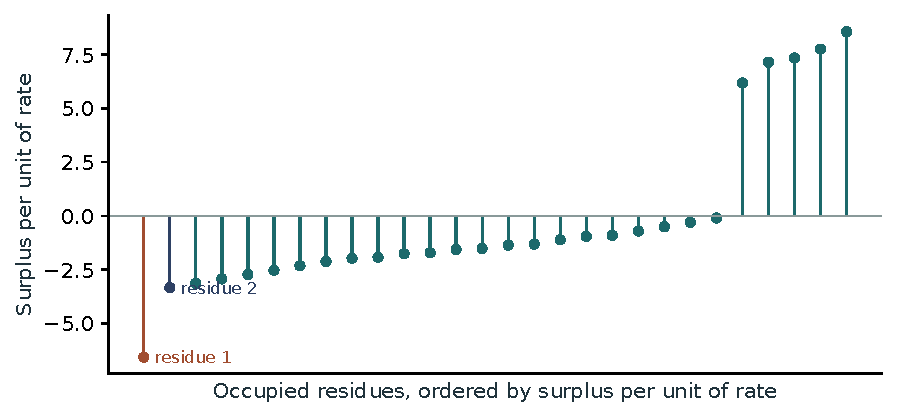
\includegraphics[width=.90\linewidth]{figures/rates.pdf}
\caption{On the adverse order of the previous support rule, each vertical segment is a leaf's coefficient \(p_t-zq_t\) at the optimized standard target. Rates should be exchanged according to differences between these heights. Leaf 1 has the lowest height but must supply marks. Leaf 2 can absorb the count adjustment.}\label{fig:rate-ledger}
\end{figure}

The large change since the previous paper came from freeing the allocation on the surviving leaves. Restoring the trial-count prefactor subsequently gains only about \(0.0000356\) percentage points. It would be misleading to ascribe the first improvement to a weakened admissibility test, or to use the second as evidence that a particular support exchange helped on every order. The next experiment changes the actual positions and keeps an explicit fallback wherever its new supports cannot certify a higher fraction.

\section{What changes when the selected residues can move?}
\label{sec:lower-support}

A lower bound for every labeling and a count of the labelings that do especially well answer different questions. The 64-cycle separates them sharply. The following construction guarantees at least
\[
             z_{\rm window}=\frac{27748320734}{274219308421}
                      =0.101190251313\ldots
\]
under the original score comparison, subject to the arithmetic transport established in this study. A second construction reaches \(11\%\) on 15,318 of 16,384 possible normalized sparse configurations, uniformly over their dense completions. The two rules can be combined by using the second when its certified margin is nonnegative and the first otherwise. This makes support selection materially useful on identifiable inputs. The evidence for the last few difficult configurations is quite different.

The distinction matters for a simple reason. A support can remove an entire difference class by deleting the last pair that realizes a shift. Lowering one endpoint from a large positive rate to a tiny positive rate never accomplishes this in the support-level certificate. Once a shift has disappeared, though, the credit still depends on how much mass remains on the odd side of the node. These two operations face different obstacles. The first is a finite question about the geometry of residues. The second must also respect the score's need for even singleton cells. We isolate their effects by recording three quantities for each tested percentage: the number of covered configurations using one sparse anchor, the number after permitting a second anchor, and how often a passing maximizing support uses a sparse mask absent from the historical menu.

\subsection{Retaining the source's whole window budget}

Write \(h=2+8\varepsilon\), \(0<\varepsilon<1/52\), and \(r=r_E(\varepsilon)\). Recall the means \(\mu\) of all sites and \(\nu\) of even sites in one candidate cell. A literal marked tile has limiting independent probability
\[
        \theta=\exp(-(6r+1)\mu)\,\nu^{3r}.
\]
The convenient sufficient inequality \(\theta>10^{-(6r+1)}\) can spend more of the failure budget than necessary. There are at least \((h+3)10^{6r+1}\log x\) disjoint trials after dropping the possible trial containing a conditioned retained point. There are \(O(x^h)\) starts. The weighted score proof asks for a per-orbit conditional failure probability \(o(x^{-2})\). Consequently it is enough that
\begin{equation}
       10^{6r+1}\theta > \frac{h+2}{h+3}.
       \label{eq:lower-window}
\end{equation}
Indeed, strictness permits a \(\theta'<\theta\) on the same side of the inequality. Each late trial has success probability at least \(\theta'\) in the comparison law. Multiplying the exponential failure bound by the number of starts gives the exponent \(h-(h+3)10^{6r+1}\theta'<-2\). The relative fixed-count comparison is applied at each start before the union. Both \(r\) and the strict margin are fixed before \(x\) increases. The derivation uses the literal window multiplicity in the source and applies to the chosen sampling argument. A better estimate of score compatibility for another law could give a different feasible set.
\href{https://github.com/nousentllc/riemann-hypothesis/blob/40e56bab026552e089d7afcfeff08d2defb9c005/src/Formalism/SharpRestriction/GrowthBounds/UnramifiedQuadraticSetting.lean#L239-L251}{Window multiplicity in the original source}.
\href{https://github.com/nousentllc/riemann-hypothesis/blob/40e56bab026552e089d7afcfeff08d2defb9c005/src/Development/AutomorphicArithmetic/ThickFrames/TilesLe.lean#L43-L67}{Trials after conditioning on one site}.

For a numerical certificate uniform over \(\varepsilon\), factor the left side of \eqref{eq:lower-window} exactly:
\[
       10^{6r+1}\theta
       =\frac{(10e^{-\mu}\sqrt{\nu})^{6r+1}}{\sqrt{\nu}} .
\]
Since \((h+2)/(h+3)<54/67\), the two rationally verifiable tests
\[
    \log 10-\mu+\tfrac12\log\nu>0,
    \qquad (54/67)^2\nu<1
\]
suffice on a tile. Their separation is deliberate. The exponent can grow without bound as \(\varepsilon\) decreases. A base strictly below one cannot be offset for all \(\varepsilon\) by a fixed prefactor. Conversely a base slightly above one, accompanied by a suitable prefactor, already controls every finite exponent. This explains both the gain and its small size: the asymptotic leaf constraint itself moves very little.

In the exceptional frozen support give 26 ordinary high-rate leaves \(c=2.392096615\), the even singleton of the sparse half \(b=0.706267\), and the minimum of the six-leaf dense-quarter pattern \(a=64-26c-b=1.09922101\). There are 23 distinct pairs of linear forms for the two means across all three permissible reservoir deletions and all depths. Twenty-two satisfy the ordinary strict product test, checked with rational logarithm enclosures. The remaining pair is precisely \((c,c/2)\). Both inequalities above hold for this pair. Every rate is positive and less than \(12/5\), so the separate upper-count estimate used in the score transfer continues to apply. The finite geometry from the fixed-support analysis gives
\[
                 \frac PQ\ge\frac{116c}{2112+254c+32b}
                    =z_{\rm window}.
\]
The ordinary charts give at least \(11661/115010\), which exceeds the displayed floor. The rational parameters have deliberately retained strict margins. This certificate provides a counterexample to treating the optimum of the standardized tile test as the optimum for the literal source score. Its improvement over the strongest frozen standardized certificate is about \(0.00003555\) percentage points. The preceding section approaches the same literal corner more closely with sharper rational rates. The wider margins here provide a shorter independent check before the support experiment.

\subsection{An exhaustive sparse-coordinate experiment with explicit quantifiers}

Denote by \(E,O\) the preferred and opposite halves of the root. Decompose their children in canonical order as \((A,B)\) and \((C,D)\), respectively; each has width 16. The letters in this section always refer to these four quarters. In \(A,B,D\) permit every nonempty canonical mask satisfying the local even-mass tests described below. In \(C\), retain its own minimum and optionally the minimum in its opposite child. Each positive scaled rate belongs to
\[
            \{1/8,2/8,\ldots,19/8\}.
\]
The total is 512 eighths. This finer control of the locations and coarser choice of the rates are independent design choices. In particular, this family can fail just below the continuous fixed-support certificate. Falling back on that certificate keeps the all-label result.

Give \(O\) coordinates in \(\mathbb Z/32\) with the \(C\) minimum at zero and multiply by the inverse of the coordinate of the \(D\) minimum to put it at one. Its oddness makes the inverse available. The selected \(C\) coordinates are \(2S\), where either \(S=\{0\}\) or \(S=\{0,s\}\), with \(s\) odd modulo 16. The \(D\) coordinates are \(1+2T\). The recursive canonical order on a 16-cycle comes from 15 binary choices. Of the resulting \(2^{15}\) orders, exactly 2,048 have their first entry at zero, the condition on the coordinate list of \(D\). Every odd \(s\) can occur separately for each such order since the two subtrees of \(O\) have separate choices. Hence the experiment tests \(2{,}048\cdot8=16{,}384\) sparse configurations.

Within either dense quarter, shift its first canonical point to zero and multiply the odd difference to its opposite-child minimum by its inverse. The conditions on canonical entries 0 and 8 reduce the number of orders to \(2^{15}/(16\cdot8)=256\). The affine change preserves addition of steps, the number of missing steps at each depth, and canonical odd mass. Different dense quarters may choose different normalizations because the conservative search takes zero recovery credit at the width-64 root and at the width-32 node \(E\). It still charges their entire odd exposure. This is what makes a bound for the two independently normalized quarters applicable to every completion in the physical cycle. To credit root recovery one would also have to align their actual relative coordinates.

Let \(T\) now denote the occupied coordinate set within \(D\). The digits \(j\) corresponding to the allowed odd increments \(1+2j\) in \(O\) are exactly
\[
                   (T-S)\ \cup\ \{-1-k:k\in T-S\}.
\]
Taking differences from a point of \(2S\) to a point of \(1+2T\) gives the first set. Taking differences in the opposite direction gives the second. Thus the number \(d_O\) of missing increments is 16 minus the size of that union. The second anchor can enlarge the union, which reduces the return on every tick in \(D\). Locally inside \(C\) the two anchors have opposite parity. They realize exactly two distinct odd differences, \(s\) and \(-s\); the other six odd differences in that 16-cycle are missing. The extra gain for mass on the second anchor is therefore 12 times its mass. If the two new translated difference sets contribute no previously uncovered digit to the union, the additional anchor earns this local gain with no reduction in \(d_O\). If they cover several new digits, a singleton can be preferable. The search takes both possibilities seriously.

\subsection{A threshold computation that preserves the signs}

At target \(z=p/q\) write the integer margin as \(qP_8-pQ_8\), where the subscript denotes rates in eighths. Clearing denominators lets all geometry and all threshold decisions use integers. Inside a quarter the coefficient of a single tick at canonical rank \(i\) is
\[
 2q\!\sum_{\substack{v\text{ internal to the quarter}\\i\text{ in its odd child}}}\!d_v
                     -p(1+2i).
\]
Indeed, the weights of the binary digits of rank \(i\), doubled, are exactly the widths of the internal nodes where its branch was odd; the extra one accounts for the leaf tail. Every \(B\) tick pays another \(32p\), and every \(D\) tick adds \(2q d_O-96p\). The first \(C\) anchor contributes \(-65p\) per tick and the second contributes \(12q-81p\). In particular dropping parent recovery never removes its exposure from the denominator.

To obtain a reusable finite constraint on marks, take an occupied local node of width \(w\), \(n_v\) active leaves and total mass at most \(19n_v\) ticks. Use the upper mean \(19n_v/(8w)\) in the factor \(e^{-\mu}\). Require the even-child tick count \(u\) to be at least the smallest integer for which
\[
         e^{-19n_v/(8w)}
         \min\left\{\left(\frac{u}{8w}\right)^{1/2},
                    \left(\frac{u}{8w}\right)^{6/13}\right\}>\frac1{10}.
\]
The two exponents bound the source interval since \(r\ge2\). For a given width and total, the checker encloses the exponential by a Taylor partial sum and a geometric upper bound on the positive remainder. It verifies that the first passing integer clears the upper endpoint and its predecessor fails even at the lower endpoint. The code also checks every homogeneous leaf rate; otherwise all coarse nodes could pass while the increasingly fine levels fail. In the two upper levels and in the sparsely occupied \(C\) quarter it checks the mark again at the actual masses. Exactly 1,806 of the 65,535 nonempty quarter masks survive the conservative local test.

This organization makes changes in mass cheap to evaluate. Give an active leaf one tick to retain its support. Visit the mandatory even-subtree floors from the smallest nodes upward. To discharge a deficit add available ticks in that subtree in descending order of margin coefficient. A later addition can only help earlier lower bounds, since the assumed total in the exponent was already at the support maximum. After all floors pass, fill remaining capacity in descending coefficient order and record one feasible objective at every total reached. The certificate needs only the feasibility and the achieved objective of these allocations. Stronger constraints from the worst total may discard arrays whose actual marks would pass. In particular a negative outcome of this routine cannot upper-bound all profiles on its chosen support.

For a dense order \(L\), let \(V_L(m)\) be the best margin offered at total \(m\) in its quarter. Take the pointwise lower envelope \(V(m)=\min_L V_L(m)\). At given combined dense total \(e\), every dense completion can guarantee
\[
  W(e)=\max_{a+b=e}\{V(a)+V(b)-32pb\},
\]
with the mark required at \(E\). A maximizing split \((a,b)\) is universal at that total, while the two winning internal supports may depend on their own orders. Combining \(W\) with each sparse configuration and both choices of \(S\) yields a lower bound before reading the dense part of the labeling. The finite operations are in this order because choosing a different favorable dense order for each mass would answer the wrong quantifier. The minimum inside the envelope makes the certificate conservative and suggests a precise check when a sparse configuration misses its target.

\subsection{Where the additional support pays for itself}

The following counts refer to the normalized \((D,s)\) coordinate pairs just defined. A passing count applies to every dense completion of that pair. The last column counts passing cases in which the chosen maximum uses a \(D\) mask outside the union of all eleven masks in the preceding decision rule. Ties are resolved by the enumeration order. The count identifies actual use of a new mask; it does not establish that no historical mask could also have cleared the same threshold after the other quarters changed.
\begin{center}
\begin{tabular}{@{}rrrrr@{}}
\toprule
Target & Single anchor & Either anchor rule & Additional passes & New \(D\) mask\\
\midrule
\(10.12\%\) & 16,336 & 16,369 & 33 & 14,035\\
\(10.30\%\) & 16,328 & 16,364 & 36 & 14,018\\
\(10.50\%\) & 16,288 & 16,328 & 40 & 14,001\\
\(11.00\%\) & 15,152 & 15,318 & 166 & 13,585\\
\bottomrule
\end{tabular}
\end{center}
At \(11\%\), the two-anchor option rescues 166 cases that the single-anchor component-envelope search could not certify at the same threshold. For one such layout the literal physical witness uses the following rate ticks. In \(A\) take rate 19 on all 16 leaves. In \(B\) give rank 0 rate 16, and ranks \(8,10,11,12,13\) rate 19. In \(C\) take rates 2 and 19 on ranks 0 and 8. In \(D\) give ranks \(0,4,8,12\) rate 19. The four quarter totals are \(304,111,21,76\), summing to 512. The positive \(B\) ranks in the saved physical layout correspond respectively to \(2,6,22,54,14,46\) modulo 64. The positive \(C\) and \(D\) coordinates are \(1,5\) and \(3,11,7,15\).

As a hand check, the two normalized sets are \(S=\{0,1\}\) and \(T=\{0,1,2,3\}\). Their difference digits run from \(-1\) to 3. After adjoining the reflected digits they run from \(-4\) to 3 modulo 16. The other eight digits give the missing odd increments in \(O\). Thus its recovery is \(2\cdot8\cdot76=1216\) ticks. The next level contributes \(2\cdot2\cdot95\) in \(B\), \(2\cdot6\cdot19\) in \(C\), and \(2\cdot4\cdot38\) in \(D\), or 912 in total. Two width-eight nodes contribute 76 each. The global root and dense parent have no blocked steps. Detailed allowance charges can be checked without summing individual leaf coefficients:
\begin{center}
\begin{tabular}{@{}lrrrrrrr@{}}
\toprule
Contribution & 64 & 32 & 16 & 8 & 4 & 2 & Tail\\
\midrule
Recovered ticks & 0 & 1216 & 912 & 152 & 0 & 0 & 0\\
Allowance ticks & 6208 & 5984 & 4864 & 1824 & 760 & 380 & 512\\
\bottomrule
\end{tabular}
\end{center}
Their ratio is \(2280/20532=190/1711=11.104617\ldots\%\). An independent replay reads the physical coordinates in the witness, subtracts each possible odd step at every occupied node, checks the actual quantitative marks, and agrees with the threshold search on its integer margin \(100(2280)-11(20532)=2148\). This example also illustrates why root recovery alone is a poor measure of a profile's quality. Here three smaller widths carry the full numerator while every width contributes to exposure.

\subsection{Taking apart the fifteen failures}

At \(10.12\%\), fifteen of the 16,384 sparse configurations fail the pointwise lower-envelope test. To distinguish a difficult geometry from loss through the order of the extrema, retain the entire curve \(V_L\) of each dense order. For each missed sparse configuration, first compute \(J(e)\), the best sparse contribution at residual dense total \(e\) over the same admissible one- and two-anchor choices. Combine it with every ordered pair of dense orders, now testing the sign of
\[
 \max_{a,b}\{V_{L_A}(a)+V_{L_B}(b)-32pb+J(a+b)\}.
\]
The actual mark at \(E\) is required for each tested split. This allows the split to depend on the dense orders. Pointwise-identical payoff curves can be processed together with their exact multiplicities. The 256 normalized orders give 121 distinct curves at this threshold, and the sum of products of multiplicities is exactly \(256^2=65{,}536\).

The complete Cartesian computation recovers 65,280 of the 65,536 dense completions for \emph{each} of the fifteen former misses. Thus this two-anchor family covers at least \(2^{30}-3{,}840\) of the \(16{,}384\cdot256^2=2^{30}\) normalized joint chart tuples at \(10.12\%\). This count carries more information than a further decimal place on a uniform guarantee. Nearly all the apparent failures resulted from making the dense total insensitive to the labels. The 256 remaining ordered pairs in each row all have the same \(B\) order and permit every one of the 256 orders on \(A\). The sole normalized list on \(B\), number 11,776 in the enumeration, is \((0,8,12,4,14,6,10,2,1,9,5,13,3,11,7,15)\). This locates the geometric obstruction in a specific dense quarter, even after allowing each dense order its own split.

The fallback from the fixed-support experiment localizes the survivors further. Reflect \(D\)'s first eight canonical physical coordinates about the \(C\) minimum. In normalized coordinates this sends \(j\) to \(-1-j\bmod16\). Consult the historical rule unless this reflection pairs the first eight canonical ranks with the last eight in reverse order. In the reversed case write the first eight coordinates as \(2\operatorname{rev}_3(g(i))\). The historical exceptional decision requires its free switch bits at indices \((2,4,5,6)\) to be \((0,1,1,0)\). The other bits are fixed because \(g(0)=0\). Reversing the three bits of each coordinate reproduces
\[
    g=(0,1,3,2,5,4,6,7).
\]
Hence the sole exceptional sixteen-coordinate list is
\[
 (0,8,12,4,10,2,6,14,1,9,13,5,11,3,7,15).
\]
An independent pass through all 2,048 normalized lists confirms exactly one such list. It is order 10,320 in the saved enumeration of all width-16 orders. This classification uses only the \(D\) order relative to the first \(C\) anchor. Neither the position of the permitted second anchor nor the two independently normalized dense quarters affects the historical case split. Of the fifteen residual sparse configurations only three have this \(D\) list, with \(s=3,5,7\). In the other twelve the ordinary frozen guarantee already exceeds \(10.12\%\).

It follows that the combined certificate reaches \(10.12\%\) on at least \(2^{30}-3\cdot256=1{,}073{,}741{,}056\) normalized tuples. Every realization of a passing tuple enjoys the guarantee. The count expresses coverage of a combinatorial classification. Arithmetic label frequencies and independence are unnecessary for the assertion and are unknown here. On the remaining 768 tuples the fallback still gives the all-label bound. A matching upper bound for these residual tuples would have to allow alternative \(C\) supports, broader rates and the physical alignments discarded by the two independent dense normalizations. The exact count of residual tuples supplies a finite target for that work.


We ran one more targeted test on these residuals. Keep \(B\) at order 11,776 and \(D\) at 10,320. For each of the three steps read the complete \(C\) order, of which there are 256 possibilities after fixing its two marked coordinates. Permit every structurally compatible \(C\) mask with up to eight leaves and every such \(D\) mask with up to nine. Give all active leaves 19 ticks except each quarter's minimum, independently allowed every positive tick count through 19. For each candidate subtract the actual physical differences in the 32-cycle \(O\), recheck local marks at the actual rates, and combine the result with the known \(B\) order and the universal dense-\(A\) curve. All 768 detailed sparse configurations returned the same best integer margin, \(-136{,}968\) for target \(1012/10000\). Here the 768 configurations index three steps and 256 \emph{internal C orders}; the preceding residual count of 768 indexed those steps and 256 \emph{A orders}. The two counts describe different tests. This failed extension identifies a reason to change the next search: allowing more positive leaves while tying all their non-minimum rates to the cap did not recover a single additional configuration. For a particular surviving chart, interior rates or additional root credit could still help. The adverse-word calculation later shows why such per-chart improvements cannot certify 10.12 percent uniformly within the marked family.

\begin{figure}[htbp]\centering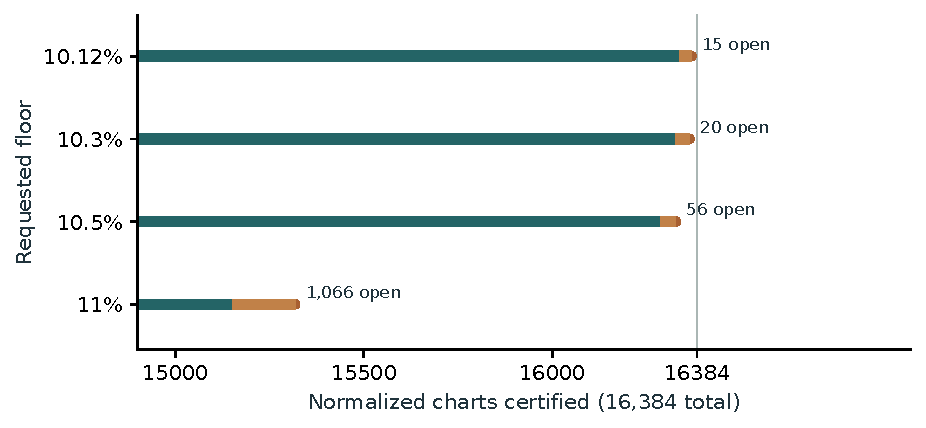
\includegraphics[width=.92\linewidth]{figures/coverage.pdf}
\caption{Support search before the finer dense-completion check. The green segment ends at the one-tip result; the short orange extension adds the second option. Each count is uniform over the unspecified dense completions of that sparse chart.}\label{fig:coverage}
\end{figure}
\section{What occupancy counts can tell us about cyclic differences}
\label{sec:geometry}
Why is the search sensitive to a change of coordinates? A useful control is to erase the actual positions at every split and give the optimizer the best local arrangement consistent with the two counts. If the resulting upper bound stays close to the observed recovery, a count-based proof might suffice. If it rises sharply, an accurate obstruction must retain some of the underlying additive geometry. To make the control informative, we first solve the \emph{local} count problem exactly.

\subsection{A sharp one-node bound}
Consider a node of width \(2m\), with \(m\) a power of two. Write its occupied physical even leaves as \(2E\) and its occupied physical odd leaves as \(2O+1\), where \(E,O\subseteq\mathbb Z/m\) have cardinalities \(e,o\). Swapping the names of the physical children only reverses a choice of coordinates. Index an odd increment by \(j\) when it equals \(2j+1\). In the first direction the allowed index set is \(D=O-E\). In the reverse direction it is \(-1-D\). For \(e,o>0\) the exact minimum number of allowed directed odd increments is
\[
 L_m(e,o)=\min\!\left(\{m\}\ \cup\
 \left\{2s\left\lceil
 \frac{\lceil e/s\rceil+\lceil o/s\rceil-1}{2}\right\rceil:
             s\mid m,\ s<m\right\}\right).                  \tag{D}
\]
If either set is empty, the answer is zero. In particular, at width two with both children populated the answer is one. The exceptional full-group term in (D) handles this smallest cycle.

For the lower inequality, let \(H\) be the stabilizer of \(D\) under translation and write \(|H|=s\). If \(H\) is the entire group, \(D\) fills the group. Otherwise \(D\) is a union of cosets of \(H\). In the quotient, Kneser's addition theorem gives at least
\(\lceil e/s\rceil+\lceil o/s\rceil-1\) such cosets. Indeed \(E+H,O+H\) occupy at least the indicated ceiling counts, and \(O-E\) has trivial stabilizer after passing to the quotient. Both \(D\) and its reflected translate are unions of these cosets. Reflection is \(j\mapsto-1-j\) on the quotient of even order. Its fixed-point equation \(2j=-1\) has no solution. Consequently the union of allowed cosets has even size, at least the least even integer above the Kneser lower bound. Multiplication by \(s\) and minimization over possible stabilizers give (D) as a lower bound. \href{https://arxiv.org/abs/1303.3539}{M. DeVos, A short proof of Kneser's addition theorem for abelian groups}.

For attainment, take a minimizing proper divisor \(s\). Set \(a=\lceil e/s\rceil\), \(b=\lceil o/s\rceil\), \(k=a+b-1\), and \(l=\lceil k/2\rceil\). In the quotient, place \(E\) in \(a\) consecutive cosets beginning at zero, and \(O\) in \(b\) consecutive cosets beginning at \(a-1-l\). Their differences lie in the quotient interval from \(-l\) to \(k-l-1\). Both this interval and its reflection fit inside \([-l,l-1]\). In each family fill the cosets until the prescribed number of individual points is reached. Truncating the last coset cannot introduce a new difference. The constructed union has at most \(2ls\) elements. The previously proved lower bound forces equality when \(s\) minimizes (D). If the minimum is \(m\), any sets of the given sizes already attain it by the lower bound. The construction proves a local sharpness statement, simultaneously for all dyadic widths. A family of locally sharp configurations need not glue to a single support.

For example, let \(m=8,e=o=2\). If \(E=O=\{0,4\}\), then \(D=\{0,4\}\) and its reflected translate is \(\{7,3\}\). Four increments are allowed, attaining (D). A one-direction count would have permitted the answer two. It would grant six missing increments when this arrangement has four. Some sets with the same counts have more allowed increments: take \(E=\{0,1\}\) and \(O=\{2,4\}\), with differences \(1,2,3,4\) and reflected indices \(6,5,4,3\). Six of the eight increments are now allowed. The change comes entirely from additive positions. Similarly, one occupied point on each side at width at least four necessarily opens two directed increments. Concentrating both at the cheapest label ranks cannot reverse that fact.

\subsection{From a local theorem to an outer problem}
At every node replace its true missing count by the generous quantity \(d^*=w/2-L_{w/2}(e,o)\). Continue to require an occupied canonical even child in every occupied node. Allow the optimizer to choose the two children's count states, including the orientation, independently of physical coordinates shared with other nodes. For a fixed declared support the numerator has only increased and the denominator is unchanged. Maximizing the relaxed fraction over every possible tree therefore bounds every fixed-label stationary marked construction with rates below a specified cap \(c\).

This apparently modest relaxation has an important order. The variables \(e,o\) count structural leaves, including possible leaves of zero limiting rate in a fixed-support closure. The mass in each child separately enters both \(P\) and \(Q\). A cap does not identify these two numbers. At fixed structural choices and trial level \(z\) the new objective is still linear in the rates, so an optimal closed-box vertex has \(\lfloor64/c\rfloor\) saturated leaves and one residual leaf if \(64/c\) is nonintegral. When the division is exact no residual leaf is needed.

This yields an exact finite recurrence. A state stores the width, number of structural leaves, number of full rates, and presence of the residual rate. To combine two child states, add both optimal child surpluses and
\[
 (2d^*-zw)\bigl(c\,k_{\rm odd}+
                    \rho\,j_{\rm odd}\bigr),\qquad
 \rho=64-c\lfloor64/c\rfloor .
\]
At the leaves include the tail charge \(-za_t\); at the root accept total mass 64. The coefficients of this recurrence are rational at a rational threshold. Updating the threshold to the attained ratio strictly raises it until the maximum surplus is zero. There are only finitely many integer state combinations. This gives the exact optimum of the count relaxation. In particular, independently choosing each best geometry cannot somehow make this an arithmetic lower certificate: each of those best choices was granted to the optimizing player.

\begin{center}\small
\begin{tabular}{@{}rrr@{}}\toprule
Rate cap \(c\)&Both directions, exact upper&Only one direction, percent\\\midrule
\(1\)&\(0\)&0.00\\
\(3/2\)&\(63/788\)&11.28\\
\(2\)&\(20/153\)&49.21\\
\(9/4\)&\(1260/6331\)&49.39\\
\(19/8\)&\(3988/14509\)&49.92\\
\(12/5\)&\(628/2277\)&49.93\\
\(3\)&\(966/2153\)&54.37\\
\(4\)&\(108/205\)&73.77\\
\bottomrule\end{tabular}
\end{center}
\begin{figure}[htbp]\centering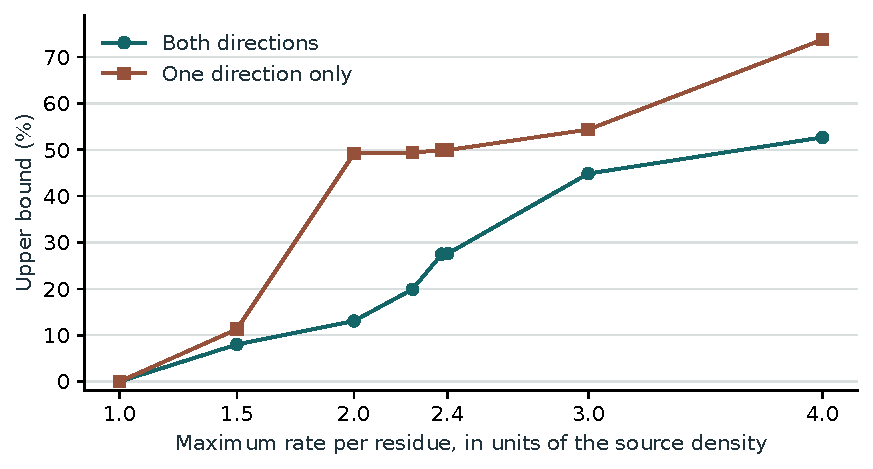
\includegraphics[width=.91\linewidth]{figures/geometry.pdf}
\caption{The exact finite optimum after forgetting joint additive placement. The larger values in the one-direction control quantify a specific accounting error. Neither curve supplies a construction.}\label{fig:geometry}
\end{figure}

\subsection{What survived the erasure}
At \(c=1\) every leaf must be filled at rate one. The vanishing result tests the orientation logic, the total and the possibility of an empty subset. At \(c=2\), the sharp local formula lowers the relaxed ceiling from \(31/63\) to \(20/153\), a change of more than 36 percentage points. At \(12/5\), counting both directions still gives \(628/2277\), roughly \(27.58\%\). The adverse-label enumerations elsewhere in this paper take this far lower. Thus a sharp one-node theorem and every tree occupancy constraint are collectively insufficient for a close estimate at the design cap.

The upper change with \(c\) is also informative. When \(c=2\), at least 32 leaves must carry mass, whereas a cap of \(12/5\) requires only 27. Freeing five leaves creates many opportunities for a difference to disappear. Those opportunities are coupled: omitting a residue to erase one increment changes which preferred minima remain in several other nodes. The separate count recurrence does not pay for incompatible physical placements. This identifies which information a more economical upper proof has to retain.

There is a separate use for a relaxed occupation bound. For a stationary exact-count profile on the conductor-one host, the good-orbit interval sum at a fixed cell bounds each class rate by \(6\mathrm e+o(1)\). To see the rate scale, sum the upper bound \(N_1\) for a window of length \(G'\) over all starting points. Every retained site is then counted \(G'\) times. At fixed depth the cell length greatly exceeds \(G'\), and \(N_1/(G'\delta)\to6\mathrm e\). A cell exceeding this bound by a fixed amount would contribute a positive fraction of the retained set on bad orbits for a positive-weight generator class, contradicting the selector's bad-mass requirement. The prior occupancy study supplies this fixed-depth argument. \href{https://github.com/nousentllc/riemann-hypothesis/pull/10}{Odd-position occupancy study}.

The extra positive-preferred-child condition in this recurrence still matters for the interpretation of that broad comparison. On an occupied long cell with no preferred retained sites, a tile requiring an even mark cannot succeed; a positive-density stationary cell would then contradict the bad-mass condition by the same fixed-depth argument. For stationary exact-count profile families with those occupied preferred children and with all allowed edges realized in the sense of Section~\ref{sec:arithmetic-transport}, \(c=16.31>6\mathrm e\) gives \(34251/39944\), about \(85.75\%\). This deliberately weak number belongs to a wider class. It explains why an upper near ten percent for strict marked profiles cannot simply be promoted to all conceivable source witnesses. A nonstationary hierarchy can evade the fixed-resolution edge-realization description.

The replay exhausts every ordered pair of subsets at group orders \(1,2,4,8\), including all \(65{,}536\) pairs at order eight. It also builds an attaining pair for every one of the \(1{,}497\) occupancy pairs across orders through 32. The first experiment checks the independent lower direction on small instances. The second checks sign conventions in the construction at the actual resolution and exercises every integer input of (D) used in the final calculation.

\section{A ceiling that tests every support on one labeling}
\label{sec:closed-box-oracle}

A successful construction gives the adversary its choice of labeling and responds with a support and rates. An upper bound reverses the laboratory procedure. We choose the labeling first, give the responding construction every support, and ask for its greatest possible advantage. A numerical optimizer that returns a good support has answered the lower-bound question a second time. To answer the upper-bound question one must either eliminate the other supports or prove that their contributions cannot exceed the proposed ceiling.

Our first ceiling applies to fixed 64-period profiles with mean-one inclusion multipliers at most \(12/5\). A supported leaf has a fixed positive multiplier in the arithmetic scale limit. We assume abundant realized edges on every significant long orbit where the periodic support permits an edge, as in the fixed-count construction. Under this condition, missing increments account for the limiting recovery numerator. Its denominator includes the unresolved finer-level allowance inside each active residue. These qualifications identify which optimization is being bounded. A class that can realize systematically few edges within a positively populated pair of residue classes needs a different upper argument. The literal window-score theorem alone does not impose the chosen pointwise cap.

\subsection{Encoding the adversary}

Give \(\mathbb Z/64\mathbb Z\) an additive coordinate. The node denoted by \((s,c)\) consists of residues congruent to \(c\bmod s\), where \(s=1,2,4,8,16,32\) and \(0\le c<s\). Its width is \(w=64/s\). In the adverse word \(W\), bit \(s-1+c\) selects the preferred child. A zero chooses \(c\bmod 2s\), and a one chooses \(c+s\bmod 2s\). Preference is defined by the least numeric label in the node. Every one of the \(2^{63}\) words occurs under some labeling. To construct one, visit all leaves of the preferred child before any leaf of its sibling, recursively. This construction also supplies a concrete permutation for an upper-bound witness.

For a support \(S\), let \(d_v(S)\) count the directed odd increments in the local \(w\)-cycle that join no two occupied leaves of node \(v\). The coefficients of a leaf \(t\in S\) are
\[
    u_t(S)=\sum_{v:\,t\text{ in odd child of }v} 2d_v(S),
    \qquad k_t=1+\sum_{v:\,t\text{ in odd child of }v}w_v .
\]
The term 1 in \(k_t\) is the mean deeper exposure in the occupied leaf. The dependence of \(u_t\) on the entire support is essential. Adding even one leaf can allow a previously absent increment, reducing the gain earned by many other leaves simultaneously. Thus applying a single linear program to all 64 rates with fixed coefficients would ignore the principal combinatorial issue.

There is a useful exact structural constraint. Every occupied node must have an occupied preferred child. If its preferred child is empty, its canonical even sites can never supply an even singleton. In the fixed-period setting the relevant step class occupies a fixed positive proportion of directions. An orbit carrying fixed positive mass in this node then fails the marked-tile test at that depth, whereas the permissible relative bad mass vanishes. Once a node is occupied, its canonical minimum must therefore belong to its support, by following its preferred children down to a leaf. This implication is much weaker than quantitative mark feasibility. It is strong enough to reduce the support search, and weakening the remaining constraints gives a legitimate upper bound.

\subsection{Why the continuous rates have a finite certificate}

Write \(z=A/C\), with integers \(A\geq0,C>0\). Because \(k_t\ge1\), the sign of
\[
           \sum_{t\in S} a_t\bigl(Cu_t(S)-Ak_t\bigr)
\]
decides whether the ratio exceeds \(z\). For its upper bound allow all \(0\le a_t\le12/5\) on the assumed support, with \(\sum a_t=64\), and drop the quantitative window inequalities. This closure can place a zero rate at a leaf still included in the geometry. That point is admissible as a relaxed certificate. A claim of attainability must separately inspect the support and the rate test.

Set \(c_t=Cu_t(S)-Ak_t\). Sort the \(c_t\) in decreasing order. If a leaf of smaller coefficient has positive rate while a higher one is below its cap, transferring as much rate as possible to the higher one weakly improves the objective. A maximizing vertex therefore gives 26 leaves rate \(12/5\) and one leaf rate \(8/5\). There must be at least 27 occupied leaves. Multiplying all rates by five, the maximum over rates on a fixed support is exactly
\[
              12\sum_{i=1}^{26}c_{(i)}+8c_{(27)} .
\]
This calculation uses integers, including at ties, and it handles unequal rates that a grid search could miss. Replacing the trial ratio by the ratio of a maximizing vertex gives a finite fractional optimization method. Each improvement has a strictly positive surplus and the vertex set is finite. For the final certificate a single exhaustive computation at the reported rational threshold suffices. An explicit vertex with surplus zero certifies equality in the relaxation at that labeling.

\subsection{An envelope for the two half cycles}

Listing all legal supports globally would be expensive. If \(b_w\) counts legal supports on width \(w\), including the empty support, then
\[
                  b_1=2,\qquad b_{2w}=1+(b_w-1)b_w .
\]
The preferred side is nonempty whenever the parent is nonempty, and the other side may be arbitrary. This gives \(b_{16}=1807\) and \(b_{32}=3{,}263{,}443\). At width 64 the recurrence already gives over ten trillion possibilities. There is no reason to bear their Cartesian product for the most common case.

Temporarily credit no recovery at the 64-leaf root. For each half, form a table \(F(k,j)\) giving its greatest threshold surplus with \(k\) full-rate slots and \(j\in\{0,1\}\) partial-rate slots. Internal gains, the leaf tail and every odd allowance at or below that half remain in the table. For fixed \(k,j\), the odd half incurs the additional root charge \(64 A(12k+8j)\). Thus the greatest surplus in the root-uncredited envelope is
\[
 \max_{0\le k\le26,\,j=0,1}
 \left[F_E(26-k,1-j)+F_O(k,j)-64A(12k+8j)\right].
\]
Edges that contribute no recovery at the root no longer couple the left and right supports. Only the total slot counts pass between halves. A zero-mass half can be padded by a required minimum at zero rate in the closed relaxation. The envelope also allows a pair of supports that accidentally do leave a root hole, in which case it undercredits their root recovery. The next sector explicitly restores the full credit on every such pair that carries odd mass, so no support is lost by this decomposition.

Computing the half envelopes follows the same logic one level down. For a base envelope at width 32, combine the independent width-16 tables and charge the canonical odd half its width-32 allowance. Then enumerate pairs of legal quarter supports that can carry a width-32 hole with nonempty odd child. There are only \(1807^2\) pairs before any overlap tests, and width-16 support data are reused. This recursion exploits the fact that an ancestor contributes the same coefficient to every unit of rate in a whole odd child. One need not communicate an entire rate vector to compute this charge.

\subsection{Accounting for every missing root increment}

For root credit to be positive the odd side must be occupied and some odd step \(h\) must be absent. We can index the search by \(h=1,3,\ldots,31\), one representative of each unsigned pair. If the occupied same-parity set is \(E\), the opposite side is forbidden from both \(E+h\) and \(E-h\). In parity-half coordinates these are two cyclic translates on 32 positions. A check in only one direction would allow the reversed edge and overstate the recovered amount.

Given an allowed set \(L\) on a subtree, its largest legal subset is unique. Construct it recursively. If the preferred child has empty legal interior, the entire interior is empty. Otherwise take both child interiors. Every legal subset of \(L\) is contained in this result, because every occupied preferred path must survive. This is a sharper necessary condition than simply counting the residues of \(L\). A hole can forbid a small number of spatial locations while forcing a much larger subtree to be empty through its minimum.

The fast search enumerates one legal preferred half, subtracts the two forbidden translates for each proposed \(h\), and replaces the allowed part of the other half by its legal interior. It discards the branch if the two halves cannot supply 27 leaves. It then lists all legal quarter submasks of that interior whose union can supply the remaining count. A support that lacks several increments is evaluated at its smallest missing unsigned increment. For that support the numerical calculation counts \emph{all} missing increments, adds the full root gain, and sorts the 27 required coefficients. Duplicate removal concerns the number of candidates examined and preserves the amount of gain credited to each candidate. The case of a wholly empty odd half has zero root credit and is covered already by the envelope.

\subsection{Independent audit by propagation of required minima}

The independent verifier represents a support as 64 bits in the original additive coordinate. It computes a prerequisite set \(P(t)\) for each leaf: the leaf itself and the canonical minimum of every node containing it. Inclusion of \(t\) forces every member of \(P(t)\); exclusion of \(s\) forces exclusion of every \(t\) for which \(s\in P(t)\). Fix a forbidden generator \(h\). In a recursive search, inserting a leaf inserts its prerequisites and excludes the two translated neighbors of each inserted point. If an exclusion reaches a prerequisite of an already retained leaf, the branch terminates. If fewer than 27 unbanned leaves remain, it also terminates. Splitting on a still undecided leaf makes these branches exhaustive and disjoint. The final mask gives the literal list of missing cyclic increments by rotation and intersection.

This verifier deliberately uses a different algorithm on the other sector as well. It enumerates all \(3{,}263{,}443\) legal supports on each half, computes their local coefficients, and maximizes the two tables by direct sorting. It shares no quarter-mask interior table with the faster oracle. Agreement on the number of multiply visited root-hole supports, the number of distinct ones and the maximum surplus in each sector provides more information than two executions of the same executable. A separate Python calculation subtracts literal residues on the winning support and checks the equality vertex.

\subsection{An equality vertex at the adverse labeling}

The word \(W=2556884934454963932\) yields a closed-box maximum of \(99/916\), approximately \(10.80786\%\). At this threshold the fast census counted 36,802 compatible support--missing-generator pairs carrying mass on both parities and 33,631 distinct such supports. The independent checker reproduced both counts. In the integer units of the threshold test \(916P-99Q\), with rates multiplied by five, the best surplus in this sector was \(-210{,}792\). In the separate envelope ignoring root credit the maximum was exactly zero. The two sectors show that any profile at this labeling lies at or below the stated cap ceiling.

The equality support has 27 leaves. Write the groups in ordinary residue coordinates as
\[
\begin{aligned}
 E={}&\{0,4,8,10,12,16,20,24,28,32,36,40,44,46,48,52,54,56,60\},\\
 O={}&\{5,25,33,37,41,47,53,57\}.
\end{aligned}
\]
Give residue 47 rate \(8/5\) and the remaining 26 residues rate \(12/5\). All rates on the displayed support are positive. Computing its ledger directly by subtraction gives the following values, expressed with rates multiplied by five.
\begin{center}
\begin{tabular}{@{}rrr@{}}\toprule
Node width & Recovery numerator & Odd allowance\\\midrule
64 &0 &5,888\\
32 &1,344 &3,840\\
16 &192 &2,688\\
8  &48 &1,152\\
4  &0 &528\\
2  &0 &240\\
Within-leaf tail &0 &320\\\midrule
Total &1,584 &14,656\\\bottomrule
\end{tabular}
\end{center}
For example the width-32 node on residue 1 modulo 2 misses eight odd increments and has seven full-rate leaves on its canonical odd side. Its gain entry is consequently \(2\cdot8\cdot7\cdot12=1344\). At the root even one realized adjacent orientation suffices to suppress direct recovery on a significant long orbit. This explains how the largest source of allowance on the first line can contribute no recovered gain. The maximizing relaxed support is an interior-level construction. Any scheme that counts only root holes would miss the actual obstruction furnished by this labeling.

Summing the columns gives \(1584/14656=99/916\). The equality holds in the stated relaxation at the displayed labeling. The rates on 26 leaves are at the closed-box cap, slightly above the primitive homogeneous-leaf rate allowed by the strict paired marked-cell test. Consequently this explicit vertex should not be substituted for the independently certified lower construction. It does identify the rates, positions and subtree levels on which any argument attempting to improve this upper bound must exert additional force.

\subsection{Distinguishing discovery from certification}

The calibration at word zero, which always prefers the additive child \(c\bmod 2s\), gives \(56/297\) for the same relaxation. The literal layout used in the preceding study to make its chosen rule tight gives \(384/2075\). Both ceilings exceed \(18\%\). This is a concrete example of the quantifier change. A labeling can be adverse for a single rule and accommodating for a different support chosen after seeing that labeling. Simply taking the historical hardest case as the adversary would have given little information about the reoptimized 64-cycle problem.

A seeded scan of 120 63-bit words alongside a control first produced a useful candidate with ceiling \(66/523\). Local changes to the preference bits yielded \(180/1649\) and then \(99/916\). Label search remains a constructive search for a counterexample to a larger uniform guarantee. It need not prove that the displayed word is the worst word. Its sole logical task is to produce one word. The exhaustive inner optimization does the work of converting that word into a uniform upper bound. The fixed-word replay and both algorithms are included so that verifying the conclusion does not require repeating the exploratory search. The earlier construction, raw host and baseline branches are recorded in \href{https://github.com/nousentllc/riemann-hypothesis/pull/14}{the original 64-cycle experiment}.

\section{How much do quantitative marks cost on an adverse order?}
\label{sec:priced}
A box-constrained upper bound is conclusive for every marked rule inside the box. Its maximizing vertex can still violate several of the quantitative constraints used to produce an arithmetic witness. There are two possibilities worth distinguishing. The maximizer might be a poor proxy for admissible profiles, leaving room for a large improvement in the upper bound simply by enforcing marks. Alternatively a nearby marked vector might almost attain the box maximum. In the second case a different adverse labeling, or a different reason that a support cannot arise, is necessary to make progress.

\subsection{First experiment: price the tile inequality}
At a tree node let \(M\) be total rate, \(E\) preferred-child rate and \(w\) width. For the standard tile test \(\mu=M/w\), \(\nu=E/w\). At an occupied node \(e^{-\mu}\nu^\beta>1/10\), where \(5190/10381\le\beta<1/2\). A weaker necessary condition, convenient because it admits rational separating inequalities, is
\[
  E/w \ \ge\ 0.00999\,e^{2M/w}.                       \tag{T}
\]
Indeed, if \(e^\mu/10\ge1\), raising that base to \(1/\beta\ge2\) gives at least its square. If the base is below one, the largest possible exponent is \(2+1/5190\). Its extra small factor is bounded below by \(10^{-1/5190}>0.999\). The arithmetic check raises both sides to an integer power and compares rationals. These two cases establish (T) for the whole exponent range.

Fix a tangency point \(u\). Convexity of the exponential gives
\[
 g=E-2bM+w b(2u-1)\ \ge0,\qquad
    b\le0.00999\,e^{2u}.
\]
To round \(b\) down safely, distinguish whether the tangent factor \(1+2(\mu-u)\) is positive. If it is negative the inequality follows already from nonnegative preferred mass. If \(u\ge1/2\) this inequality also holds on an empty cell, where \(M=E=0\). On the path to the absolute preferred leaf every node must be occupied, so positive-intercept tangents are permissible there. The distinction prevents an empty valid subtree from being accidentally penalized by a bound meant only for occupied cells.

A family of necessary inequalities \(g_i\ge0\) can certify an upper bound \(z\) if
\[
 \max_{\text{supports, closed-box rates}}
       \bigl(P-zQ+\sum_i\lambda_i g_i\bigr)\ \le0,\qquad \lambda_i\ge0 .
\]
The sign of the multiplier is positive because the outer maximization has discarded the constraints. Feasible original points add a nonnegative amount to their surplus before the maximum is taken. Each tangent is affine in rates, so it adds a leaf price and a constant to the exhaustive oracle. Round each coefficient and the constant upwards on a fine grid: every originally feasible point only gains surplus, even if some coefficients are negative. A nonpositive maximal rounded surplus still proves the claimed inequality. Floating-point linear programming proposed multipliers during discovery. Verification uses integer arithmetic and reads the published coefficients.

On word \(2556884934454963932\), at cap \(2393/1000\), this cut search returned \emph{zero} multipliers. The price-free upper threshold was \(10764/100000\), with residual \(-2414976\) in the oracle's integer units; one tick lower its residual was \(519808\). The result is useful as a failure of the proposed intervention. It does not indicate that tile constraints never matter. The next calculation explains why this particular witness left so little room for these prices to work.

\subsection{Second experiment: meet the upper from inside on this word}
Take the 27 physical residues of the equality example in Section~\ref{sec:closed-box-oracle}. Give every residue except 47 the rate
\[
 c=2.3920857150,\qquad a_{47}=64-26c=1.805771410.
\]
Compute the literal differences in every node. The 26 ordinary leaves have total coefficients \(132\) for recovery and \(1178\) for allowance. Leaf 47 earns zero recovery and pays 65 units of allowance per unit of rate. Thus the following expression reduces to \(132c/[1178c+65(64-26c)]\).
\[
 f(c)=\frac{\sum_{t\ne47}p_t c+p_{47}(64-26c)}
            {\sum_{t\ne47}q_t c+q_{47}(64-26c)} .
\]
The independent implementation evaluates each occupied-cell pair \((\mu,\nu)\) and the homogeneous test below each occupied residue. In all, 69 tests pass at this profile. The smallest lower bound on \(\log(10T_r)\) exceeds \(10^{-11}\). The strict, uniform lower value on this particular word is
\[
 \frac{15787765719}{146762605696}=10.7573490155\ldots\%.
\]
It is attainable in the sense of the family construction. In particular the small log margin does not translate into a certified numerical value of the first sufficiently late host.

Can the same word rule out \(10.76\%\)? For a profile required to satisfy the standard test at every exponent, a homogeneous leaf at rate \(a>2\) must pass \(e^{-a}(a/2)^{5190/10381}>1/10\). This expression decreases in \(a\) above two. Its failure at \(239209/100000\) therefore bounds every rate by that rational cap. Rerun the exhaustive fixed-label oracle at this cap and at the exact ratio of the above vertex with that new \(c\). Its maximal surplus is zero, including root holes and closed supports. It proves an upper bound on the original fixed-word optimum of
\[
 \frac{2631299}{24460416}=10.7573763259\ldots\%.
\]
Even allowing the profile to vary with one fixed source exponent, the weaker universal cap \(23921/10000\) gives \(789393/7338112=10.7574400609\ldots\%\). The same program certifies the homogeneous upper failure and maximal residual in each case. The positive example and the bounds surround the uniform standard fixed-word optimum within \(0.000028\) percentage points.

This is a falsifiable diagnosis of why the first approach stalls. On that order a rule really can recover nearly \(10.75735\%\) and meet the quantitative marks. No further refinement of a mathematically valid inequality for the same class and the same labeling can give, for example, a \(10.5\%\) upper bound. Searching for a better \emph{word} becomes essential. It is possible for tile constraints to be economically inactive on one order while ruling out the best entire sector of supports on another. The next comparison exploits precisely that difference.

\section{A sharper adverse labeling and a test of its surviving vertex}
\label{sec:rootmark}

The best adverse labeling in the second search gives
\[
 \sup_{\text{rules}}\inf_{\text{labelings}}
 \frac{\mathcal R}{\mathcal K}
 \ \le\ \frac{1018318}{10^7}=10.18318\%.
\]
Here a rule assigns nonnegative rates of total 64 to the labeled residues. These rates may depend on the labeling, remain fixed across \(0<\varepsilon<1/52\), and meet the limiting marked-tile product certificate, including its source-window prefactor if used. Closures of this class satisfy the same upper bound. Paired with the constructive \(10.1190251313\%\) lower result for the prefactor version, the interval before the final census is about \(0.06415487\) \emph{percentage points}. This bound applies to the quotient experiment. The original selector could admit laws that pass by a different argument.

\subsection{Two consequences of using one profile across the source scales}

For an occupied coset of width \(w\), let \(M\) denote the sum of the rates in it and \(E\) the sum in its preferred child. Thus \(\mu=M/w\) and \(\nu=E/w\). The familiar sufficient condition is
\(10e^{-\mu}\nu^{3r/(6r+1)}>1\).
The refined union bound for the literal number of trial tiles allows its \((6r+1)\)-st power to exceed \((h+2)/(h+3)\). In the original scales \(h=2+8\varepsilon\) and \(r=\lceil32/\varepsilon+64\rceil+1\). As \(\varepsilon\) tends to zero, \(r\) tends to infinity, \(3r/(6r+1)\) tends to \(1/2\), and this positive prefactor raised to \(1/(6r+1)\) tends to one. Testing a fixed vector for every \(\varepsilon\) therefore gives the necessary closed inequality
\[
 E\ \ge\ \frac{w}{100}\exp(2M/w).
 \tag{R1}
\]
This is a necessity for either stated certificate across the scales. It does not assert the inequality for a vector allowed to change with \(\varepsilon\) in the refined test.
\href{https://github.com/nousentllc/riemann-hypothesis/blob/40e56bab026552e089d7afcfeff08d2defb9c005/src/Development/AutomorphicArithmetic/ThickFrames/MarkedLow.lean#L20-L31}{Original parameter definitions}.
\href{https://github.com/nousentllc/riemann-hypothesis/blob/40e56bab026552e089d7afcfeff08d2defb9c005/src/Formalism/SharpRestriction/GrowthBounds/UnramifiedQuadraticSetting.lean#L237-L251}{Trial-block multiplicity}.

At the root \(M=64\), so \(E\ge0.64e^2>4.72\). In a homogeneous positive leaf with rate \(a_t\), the finer cosets give \(e^{2a_t}\le50a_t\). The ratio \(e^{2a}/a\) increases for \(a>1/2\). The fortieth-term Taylor partial sum at \(2(23921/10000)\), even with its positive remainder removed, exceeds \(50(23921/10000)\). It follows that \(a_t\le C=23921/10000\) for every leaf, including zero-rate leaves. In particular at least two preferred root leaves must carry positive mass. This observation removes an entire class of possible supports when the root itself has a missing increment. A support maximizing a relaxation that ignores root holes may still be included with fewer preferred leaves; this only enlarges that relaxation.

\subsection{Detecting occupancy by the mass of a specific leaf}

The adverse word is \(2549776587809433532\), with bit \(s-1+c\) specifying the preferred child of residue \(c\bmod s\). Its root prefers the even numbers; inside the odd coset the preferred child consists of the residues \(3\bmod4\). Consider the width-32 odd coset. If it is empty, its preferred mass is zero. In an occupied coset the exponential in (R1) has a positive tangent intercept for \(u<1/2\), so applying its tangent at such \(u\) to an empty coset would be unjustified. A leaf provides a continuous lower bound on the occupancy indicator. If \(t\) is in this coset, then
\[
 \mathbf1_{\{M>0\}}\ \ge\ a_t/C.
\]
Fix \(u=3/8\), \(t=9\), and put \(k=\lfloor 10^9 S_{39}(2u)/100\rfloor/10^9\), where \(S_{39}\) sums through power 39 in the exponential series. Then every admissible rate vector satisfies
\[
 L(a)= E-2kM-32k(1-2u)\,a_9/C\ \ge\ 0.
 \tag{R2}
\]
Indeed, on a nonempty node, bounding the exponential below by its tangent gives \(E\ge \exp(2u)[2M+32(1-2u)]/100\). Both coefficients here are nonnegative, so one may round \(k\) down and then replace one by \(a_9/C\). On an empty node all terms in (R2) vanish. The choice of \(u\) is explained by the obstructing vertex below. A single price for the preferred \emph{root} mass had little force on that vertex. Its violation is one level lower.

For any nonnegative \(\ell\), the priced objective \(P-zQ+\ell L(a)\) upper bounds \(P-zQ\) on every feasible profile. Using \(\ell=803133/10^6\), we round each coefficient of \(\ell L\) upward to units of \(10^{-7}\). All masses are nonnegative, so rounding preserves the upper direction. Enumerate the full binary-tree support family, with the root elimination above, and relax each support to a closed capped simplex. The maximum of a fixed affine function on one of these simplices places \(C\) at 26 sites, \(1.8054=64-26C\) at one further site, and zero at the others. In particular the maximization can overcount a profile by allowing a nominally occupied leaf to receive zero mass. This freedom is needed for an upper bound without an artificial minimum positive rate.

\begin{center}
\begin{tabular}{@{}lrr@{}}
\toprule
Test at the final word & Numerator of \(z\) & Scaled maximum\\
\midrule
Target, unpriced  & 1018318 & \(54\,250\,880\,988\)\\
Target, one priced node & 1018318 & \(-22\,184\,178\)\\
Previous grid point, same price & 1018317 & \(8\,175\,060\)\\
\bottomrule
\end{tabular}
\end{center}
The score units are \(10^{-11}\), from combining the \(10^{-7}\) coefficient grid and \(10^{-4}\) mass units. A negative maximum certifies the bound for the continuum of rate vectors on each support. The positive maximum one tick earlier identifies the resolution of this particular price and relaxation. It gives no matching lower construction. Three comparison words from the same search yielded bounds \(10.18996\%\), \(10.20123\%\), and \(10.56603\%\) under their recorded choices of prices. The last of these used zero prices. A weaker closed-box optimum at one labeling was therefore a poor guide to which labeled constraint would produce the sharpest result after pricing. An independent integer census gave the same two signed maxima. It used 3,263,443 admissible masks for each 32-leaf half, and found 39,058 distinct whole-group supports across 42,384 support--missing-pair incidences in its root-hole sector. The maximum there at the accepted target was \(-1{,}968{,}374{,}370{,}320\). The tighter competitor was the envelope without root-hole credit.

\subsection{Trying to turn the surviving vertex into a construction}

The final priced maximizer illustrates why the finite dual and a constructive lower bound remain distinct. After restoring the preferred leaves required by its nonzero support, its odd coset contains the six residues \(1,9,17,21,27,33\). Five receive \(C\); the preferred residue \(27\) receives zero. The actual mean in that coset is \(5C/32=23921/64000\), close to \(3/8\). Its even-site mean vanishes. Before adding any price, the geometric quotient at this vertex is about \(10.20312816\%\). Its odd coset cannot supply the required even singleton. The priced score subtracts from the objective precisely because the preferred mass is missing and leaf \(9\) is full. Retaining only the raw objective would hide the failure.

A separate constructive control started from the active vertices for five nearby prices, restored their smallest preferred-child closures, and tried changing one retained class at a time. Across 86 distinct resulting supports, a real-valued solver proposed rates, which we rounded and checked against the exact total and the strict standard tile margins using rational logarithm enclosures. The best profile in this search has the same 28-leaf closure. Its two exceptional rates are \(0.70626403\) at residue \(27\) and \(1.09955197\) at residue \(46\); its other 26 occupied leaves all have rate \(2.392084\). The odd coset now has a genuine preferred mass. On this one word the ratio is
\[
 \frac{433565225}{4284671539}=10.1189839420\%.
\]
All 21 distinct pairs of cell means pass the strict rational checks. This attained value is a diagnostic for the adverse word. The separate all-label construction supplies the stronger lower bound quoted at the beginning of this section. A small repair of the closed vertex restores an admissible geometry, but this intermediate interval alone does not tell us whether a different support beats that repaired profile or whether more occupancy constraints can exclude the competing closed vertices. The final census in Section~\ref{sec:cycle64-endgame} separates these explanations by identifying every nominal support capable of exceeding the constructive guarantee.

\section{Reducing the adverse word to two supports}
\label{sec:two-support-census}

The closed-box program can answer a more informative question than the value of its highest peak. Set the trial fraction below the known construction and ask for the identity of \emph{every} support that could clear it. If very few survive, the nonlinear marked-cell restrictions can be brought back on those supports individually. This reverses the order of work from adding a single global inequality and improves on the price bound even when its maximizing rate vector changes discontinuously.

\subsection{A change of relative phase}

The decisive word is \(W=2549776587809433532\). It arose from the sampling and recombination of labeled 32-leaf halves, followed by a change of coordinates on one half. There is a useful control with an exact geometric interpretation. Start at word \(7382425669205845932\). Keep all even physical leaves fixed. In the ranking of the odd leaves \(2y+1\), replace each \(y\) by \(11y+6\bmod 32\) and transport the rankings with the leaves. Keep the even half preferred at the root. Reading off preferences from the resulting rankings gives \(W\).

Multiplication by \(11\) permutes the odd directions on the 32-cycle and its dyadic quotients. Translation permutes the residue nodes. Consequently the two odd-half problems have identical gain and allowance data after relabeling, including their preferred children. Their relative positions with respect to the \emph{fixed} even half have changed. In the two-sector relaxation with cap \(12/5\) and at least two preferred root leaves in its missing-step sector, the original word gives \(32/187\) and the transported word gives \(58/567\). This large drop is a root effect. It shows why optimizing each half and accepting the first interleaving of their coordinates leaves an important decision uncontrolled.

\subsection{All supports above a threshold}

Fix \(z=10118/100000\), corresponding to \(10.118\%\). Two cap enclosures will be useful,
\[
  C_1=23921/10000,\qquad C_2=239213/100000.
\]
In each case a vertex for fixed structural support has 26 leaves of rate \(C_j\) and one leaf of rate \(64-26C_j\). Structural support here means all leaves regarded as occupied when calculating edge availability. A leaf in that support may carry zero mass at an optimizing vertex of the closure. The enumeration keeps these leaves as occupied. This detail is essential when an argument is to exclude all supports with positive rates as well as their independently optimized boundary vertices.

Let \(H_B(A,k,j)\) be the best contribution of the individual half mask \(A\) on side \(B\) when \(k\) full slots and \(j\) partial slots are placed there. Include the root \emph{charge} in the odd half and temporarily credit zero root gain. The best possible completion in the opposite half is
\[
       F_{\overline B}(26-k,1-j)=
       \max_{A'} H_{\overline B}(A',26-k,1-j).
\]
A necessary condition for a positive surplus on \(A\) is
\[
        H_B(A,k,j)+F_{\overline B}(26-k,1-j)>0.
\]
Apply this filter to all 3,263,443 legal masks on each side, separately for each slot split, then form the actual cross products of the two surviving lists and check their sums. This last check prevents two half masks found using different best completions from being credited with a positive joint surplus by mistake.

There are two positive full masks. Both use the same slot split at both cap enclosures. The physical even half carries 21 full slots and the partial slot. The odd half carries the five remaining full slots. Exactly two even masks and one odd mask clear the opposing-envelope filter at that split. Both compatible pairings have positive surplus. In the distinct sector where a root step is missing, the full-credit calculation examined 42,384 compatible support--direction pairs, comprising 39,058 distinct supports with odd mass and at least two preferred leaves. Even its best surplus was negative. The cap proof and the preferred-root mass constraint justify these relaxations within the stated marked-cell model.

\begin{center}\small
\begin{tabular}{@{}lrr@{}}
\toprule
Greatest \(P-zQ\) in the indicated class & \(C_1\) & \(C_2\)\\
\midrule
Missing root step, credited & \(-26.536285548\) & \(-26.5321517244\)\\
First surviving mask, root uncredited & \(0.378878364\) & \(0.3815630892\)\\
Second surviving mask, root uncredited & \(2.315139788\) & \(2.3178487964\)\\
Best other mask, root uncredited & \(-3.191590756\) & \(-3.1863520468\)\\
\bottomrule
\end{tabular}
\end{center}

All decimals in this table are exact. Integer arithmetic multiplies \(P-zQ\) by the denominator of the cap and by \(100000\). The first and second surviving masks are \(1230983613671479063\) and \(1518083709116552983\), with bit \(t\) denoting residue \(t\). Each has 28 leaves. The same distinct support \(1518085900086613781\) maximizes the uncredited envelope after removing the two winners at either cap. Thus the separation from all other supports is visible as a finite signed margin.

\subsection{A second computation after removing the winners}

An independent calculation avoids the opposing-envelope filter. It enumerates legal quarter masks by taking their preferred-child closure, joins the quarters into legal halves, and computes gains using the forbidden translates for the quarter pair. For each half and slot split retain the three highest scoring, distinct masks, with any consistent way of breaking ties. Join the resulting short lists and forbid the two specified full masks. This computes the exact best remaining surplus.

To see why three suffice, hold an opposite mask fixed. At most two masks on this side could complete it to one of the two forbidden full supports. Thus at least one of the three highest entries is compatible with the exclusion. If a surviving optimum uses an entry below the top three, replace that entry without decreasing the surplus. Having made the replacement on the first side, make the same argument on the second with the new first side held fixed. The resulting admissible pair lies in the cross product of the two length-three lists. If a half has fewer than three candidates they are all present. This argument includes ties and requires no assumption that the maximizers are unique. The fourth row of the table comes from this separate optimization. Both programs are replayed by \texttt{evidence/rootmark/near.py}.

What remains is a two-support calculation with arbitrary real rates. In both supports the preferred singleton of the sparse 32-leaf half is residue 27 and the other low-cost adjustment is residue 46. The counts of recoverable directions agree in the two saturated ledgers; the first carries an additional eight units of allowance before multiplication by the common productive rate. The next argument determines how much room any redistribution of mass has once the sparse singleton must satisfy the original marked-cell constraints.

\section{Closing the common-rate 64-cycle game}
\label{sec:cycle64-endgame}

A global upper bound can be obtained from one adverse labeling if every support and every rate vector on that labeling is covered. The census on word \(2549776587809433532\) shows that only two admissible supports have a closed-box maximum above \(0.10118\). This threshold falls \emph{below} both constructive guarantees. Consequently the only unresolved task on that word is an upper bound for arbitrary rates on two particular finite supports. Each support has a single preferred leaf in its sparse half. The resulting mass constraint is sufficiently strong to close the gap.

Throughout this section a rule can read the labeling before returning its support and rates. Its response to a given labeling must be usable for every \(0<\varepsilon<1/52\). Under this convention the optimum for the literal prefactor certificate lies in the interval
\[
 10.1190251762367
 <100\,V_{\rm literal}<
 10.1190251762403 .
\]
More precisely we have an exact implicit value and a real-valued attaining policy. The interval measures the numerical evaluation of that value. The original 10.0046 percent rule used the same winning support decisions with other rates. Once these rates are optimized, the ability to change the occupied residues gives no further \emph{worst-label} gain under the stated certificate. An individual label can have better layouts. The matching upper uses the rule's obligation to handle the particular labeling in the census.

\subsection{Why exactly two calculations remain}

Record a mask by the integer with bit \(t\) set when residue \(t\) is nominally occupied. Denote the surviving masks by
\[
 S_1=1230983613671479063,\qquad S_2=1518083709116552983 .
\]
Either can retain points in 28 residue classes. On both, the odd half of the root contains \(1,9,17,21,27,33\). Only \(27\) lies in its preferred child. Write \(b=a_{27}\). The residue \(46\) in the even half will absorb the cardinality constraint. It has coefficients \((p_{46},q_{46})=(0,33)\), and the odd anchor has \((p_{27},q_{27})=(0,65)\). Here \(P=\sum_t p_t a_t,\ Q=\sum_t q_t a_t\) include the finer-level contribution through the unit term in each \(q_t\).

Let \(I=S_i\setminus\{27,46\}\) and \(J=\{1,9,17,21,33\}\). To reproduce the coefficients, at each node form all directed pair differences between the supported residues, and count the missing odd increments. Each odd child leaf acquires twice that count in \(p_t\) and the node width in \(q_t\). Simple summation gives
\[
 \begin{array}{c|c|c|c}
 & |I| & \sum_{t\in I}p_t & D_i=\sum_{t\in I}(q_t-33)\\ \hline
 S_1&26&116&262\\
 S_2&26&116&254
 \end{array}
\]
The difference of eight reflects the dyadic exposures of three even-half leaves exchanged between the two supports. These sums alone do not establish which support is worse. An allocation could give distinct weights to all 26 sites. The following coefficient inequality controls that possibility.

\subsection{The disappearing mass of the five sparse leaves}

Let \(C\) be a common cap on all leaf rates and put \(Y=\sum_{t\in J}(C-a_t)\). The sparse half has total mass \(b+5C-Y\) and preferred mass \(b\). For a rate vector valid at every exponent, its limiting mark requires
\[
 b\ \ge\ 0.32\exp\{(b+5C-Y)/16\}.
 \tag{E1}
\]
For \(s\in[0,5C]\) let \(B(s)\) be the small positive solution of \(B=0.32\exp\{(B+s)/16\}\), and write \(B=B(5C)\). The function \(b\mapsto b\exp(-b/16)\) is strictly increasing up to \(16\). All relevant \(b\) are below \(C<2.4\), so (E1) implies \(b\ge B(5C-Y)\). Implicit differentiation gives \(B'(s)=B(s)/(16-B(s))\). At both caps used below, the exact enclosures give \(B(5C)<0.71\), hence \(0<B'(s)<1/15\) throughout the interval. Integration yields
\[
 B-b\ \le\ Y/15.
 \tag{E2}
\]
This is the quantitative reason a rate reduction on the five sparse leaves cannot pay for moving appreciable mass away from their anchor. It also covers the case where the anchor already receives more than \(B\).

For \(i=1,2\) define
\[
 z_i(C)=\frac{116C}{2112+D_i C+32B},\qquad
 v_t=p_t-z_i(C)(q_t-33).
\]
The hypothetical allocation that fills all 26 sites in \(I\) at \(C\), puts \(B\) on \(27\), and sends the remainder to \(46\) has \(P/Q=z_i(C)\). To compare an arbitrary allocation to it, eliminate \(a_{46}=64-b-\sum_{I}a_t\). Since \(64\cdot33=2112\), subtraction gives the exact identity
\[
 P-z_i(C)Q
   =32z_i(C)(B-b)-\sum_{t\in I}v_t(C-a_t).
 \tag{E3}
\]
The bound \(0.10\le z_i(C)\le0.11\) contains both critical ratios for both versions of the mark. For the two physical supports, direct integer coefficients give \(v_t>0\) throughout this range and \(v_t>32z_i(C)/15\) for \(t\in J\). Each difference is affine in \(z\); it suffices to check the two rational endpoints. Paying the first term of (E3) from the five sparse deficits using (E2) gives \(P-z_i(C)Q\le0\). Since \(Q>0\), the candidate is an upper bound valid for every rate allocation on this support. This is the weighted finite inequality covered by the general kernel lemma in this study, after supplying its computed coefficients and the scalar analytic bound (E2).

We can now compare supports without any assumption of equal rates in the competing profiles. The first support has a larger \(D_i\) and identical \(C,B\), hence \(z_1(C)<z_2(C)\). All other supports have maximum at most \(0.10118<z_2(C)\) by the census. Masks with no allowable preferred marker or too few positive root preferred leaves have already been excluded by necessary conditions. In particular, a search that listed only 27-leaf extremal vertices would not have justified discarding the 28-leaf nominal supports in this calculation. A positive anchor that disappears at a capped-simplex vertex can determine the true optimum over its parent support.

\subsection{The two sharp constants and the distinction between maximum and supremum}

Under the literal-prefactor criterion the homogeneous-leaf cap \(C_*\) is the larger root of \(10 e^{-C_*}\sqrt{C_*/2}=1\). Under the standard strict product criterion its cap \(C_0\) is the larger root of \(10 e^{-C_0}(C_0/2)^{5190/10381}=1\). The latter exponent is the smallest value of \(3r/(6r+1)\) in the admissible source range and is realized there. In either case write \(B_{\circ}(C)=B(5C)\) in the notation above. The census and projection give
\[
 V_{\rm literal}=\frac{116C_*}{2112+254C_*+32B_{\circ}(C_*)},\qquad
 V_{\rm standard}=\frac{116C_0}{2112+254C_0+32B_{\circ}(C_0)}.
\]
The second value is interpreted as a supremum. Its verified percentage interval is
\(10.118989577495<100V_{\rm standard}<10.118989577849\).

For the lower directions, use the policy that kept the original support decisions. The ordinary decisions exceed the higher of the two critical fractions at interior rational rates. In the exceptional decision take 26 common productive rates \(C\), one anchor rate \(B_{\circ}(C)\), and one residual rate \(64-26C-B_{\circ}(C)\). Of its 23 distinct cell types, 21 have a uniform positive logarithmic surplus on a rational rectangle containing the relevant corner; the smallest certified surplus exceeds \(0.1473\) in both evaluations. The two remaining types are the homogeneous high-rate leaf and the marked sparse half. In the prefactor case each has \(10e^{-\mu}\sqrt\nu=1\) at its exact corner. The powered left side of the literal comparison is therefore exactly \(1/\sqrt\nu\). For both relevant values of \(\nu\), verified rational bounds give \(\nu(54/67)^2<1\), while \((h+2)/(h+3)<54/67\) for every admissible \(\varepsilon\). Both literal inequalities remain strict. Thus the real rates at \(C_*,B_{\circ}(C_*)\) actually attain the common-rate guarantee. Fixed-count samples on increasingly late arithmetic hosts implement these rates asymptotically.

In the standard case the homogeneous leaf at \(C_0\) gives equality at the smallest allowed tile exponent. Taking \(C<C_0\) tending upward to \(C_0\), and choosing the anchor just above its small-root boundary, gives strict inequalities and limits to the claimed ratio. Conversely, equality in (E3) requires all 26 productive sites to be filled to their cap, because the coefficient inequalities have strict surplus. Those homogeneous sites cannot take the exact cap under the standard strict test. This explains why two numerically adjacent constants have different attainment statements.

The logical conclusion concerns a finite decision problem and its specified passage to arithmetic families. It uses the existence of compatible selected masks. Nothing in the matching lower and upper values identifies the set returned by a particular classical selection in the Lean source. A different proof of the original score, a finer quotient, or profiles whose rates vary with the source exponent define different optimization problems.

\section{If the rate can depend on the source exponent}
The guarantee derived above uses a policy whose rates work throughout \(0<\varepsilon<1/52\). The source itself fixes \(\varepsilon\) before selecting a witness. Could a policy that reads this parameter improve on the answer? The order of optimization matters in general. Here the two surviving supports make it possible to solve the fixed-parameter version for the literal prefactor test. This supplies a check on whether an additional uniformity convention is doing substantial work.

Put
\[
 n_r=6r+1,\quad \beta=3r/n_r,\quad
 h=2+8\varepsilon,\quad \ell=\frac{1}{n_r}\log\frac{h+2}{h+3}.
\]
The strict logarithmic cell test at this exponent is \(\log10-\mu+\beta\log\nu>\ell\). Define \(C_\varepsilon\) as the large root of the leaf equation and \(B_\varepsilon\) as the small root of the sparse-parent equation
\begin{align*}
 \log10-C_\varepsilon+\beta\log(C_\varepsilon/2)&=\ell,\\
 \log10-\frac{B_\varepsilon+5C_\varepsilon}{32}
                           +\beta\log(B_\varepsilon/32)&=\ell .
\end{align*}
On the local ranges of interest the first left-hand side decreases in \(C_\varepsilon\), the second increases in \(B_\varepsilon\). The worst-label supremum for the stationary, exact-count, edge-realizing class certified by this test at that \(\varepsilon\) is
\[
 F_\varepsilon=
 \frac{116C_\varepsilon}{2112+254C_\varepsilon+32B_\varepsilon}.       \tag{X}
\]
The formula describes the continuum of exponents, including the jumps in \(r=\lceil32/\varepsilon+64\rceil+1\). Interpolation of a small numerical grid would miss the integer changes.

To justify the upper bound simultaneously for this range, start from
\(\log(4/5)/10381<\ell<0\) and \(5190/10381\le\beta<1/2\). Exact logarithmic comparisons enclose
\[
 2.39208<C_\varepsilon<2.39213,\qquad
 0.7058<B_\varepsilon<0.7064 .
\]
For instance the leaf expression at \(2.39208\) with the smallest \(\beta\) exceeds zero; at \(2.39213\) even its largest endpoint falls below the lower bound on \(\ell\). For the sparse equation use the lower cap, lower singleton, and smaller \(\beta\) to bound its largest possible value at the lower singleton boundary. At the upper singleton boundary do the reverse. The smaller exponent maximizes the expression here because \(\nu<1\). These monotonicities avoid an uncontrolled interchange of the two endpoint exponents.

At the root \(\mu=1\). If only one preferred leaf is available, \(\nu\le 2.39213/64\); even the largest possible log margin at that value falls below \(\log(4/5)/10381\). Thus the root still requires at least two preferred leaves. The near-threshold census was rerun at the enlarged rational cap \(239213/100000\); the same two supports survive. Its root-hole residual is strictly negative. For each of the two masks the half's preferred singleton must meet a lower rate \(b\ge h_\varepsilon(s)\), where \(s\) denotes its five companions' rate sum. Implicit differentiation of the sparse equation gives
\[
 h_\varepsilon'(s)=
   \frac{h_\varepsilon(s)}{32\beta-h_\varepsilon(s)}<1/15
       \qquad (0\le s\le5C_\varepsilon).
\]
The last bound follows from the positive small root, its monotonic increase, the displayed rectangle, and the lower bound on \(\beta\). Hence the surplus comparison from the two-mask calculation is valid with \(C,B\) replaced by \(C_\varepsilon,B_\varepsilon\). The first mask's eight extra denominator units can only reduce its upper; the second gives (X).

For attainment in the limiting sense, on the frozen exceptional support put 26 rates just below \(C_\varepsilon\), put the singleton just above its corresponding lower root, and set the adjustment by the count. At a fixed \(\varepsilon\) the two defining equalities themselves are excluded by the strict test. Bounds uniform on the displayed rectangle verify that all the other 21 hard forms have log slack above \(0.14\) even under the standardized test. Moving into the strict region and then approaching the corner proves the lower supremum. The ordinary lower guarantee exceeds the largest possible (X) on the rectangle. In particular no new support policy is needed to attain the fixed-exponent answer to arbitrary precision.

\begin{center}\small\begin{tabular}{@{}lrr@{}}\toprule
Chosen \(\varepsilon\)& \(r\)&Worst-label supremum under (W), percent\\\midrule
\(64/3329\)&1730&10.1191110389\\
\(1/64\)&2113&10.1190959370\\
\(1/256\)&8257&10.1190436792\\
\(1/1024\)&32833&10.1190298549\\\bottomrule
\end{tabular}\end{center}
Each numerical entry was separately enclosed by rational bisection of both equations. These examples are not needed to establish (X). They show the size of the advantage at specific admissible exponents and test a point at the minimum source exponent.

Finally let \(\varepsilon\downarrow0\). Then \(\ell\to0,\ \beta\to1/2\), and the uniformly enclosed roots converge to \(C_*,B_*\). A rule allowed to read \(\varepsilon\) still cannot promise a larger fraction \emph{simultaneously} at every exponent, since its putative floor would exceed the optimal value at sufficiently small \(\varepsilon\). The common-rate construction already supplies the limiting guarantee. Thus the distinction matters for a particular preassigned exponent, but it disappears for the single robust number requested across the full family. This last statement concerns test (W); the raw scalar selector can admit stationary profiles by other arguments.

\section{What the experiments now explain together}
\label{sec:synthesis}
The initial trace followed a witness through an analytic argument. The encounter with classical choice raised an interpretive question: if the actual retained set cannot be extracted, which parts of the subsequent estimate follow for every allowed witness? The experiments have gradually reduced that question to one that can be answered, in part, by hand. The selection score enforces local counts and marked cells. The gain also depends on the presence of adjacent pairs for specific generators. Local count control and control of a difference set are distinct obligations. The same retained set can satisfy the first and leave a positive proportion of odd allowance recoverable under the second.

\subsection{The sequence of conclusions}
The first positive example guaranteed \(2/45\) with one selector-compatible family. A 32-cycle deletion rule subsequently attained \(10367/124242\) on its worst labeling, or about \(8.3442\%\). It became clear that the ranks cheapest for exposure and the residues best for suppressing edges need not coincide. The previous 64-cycle rule balanced them by keeping a dense quarter for supply and a sparse half for blocking. It passed ten percent by a small explicit surplus on its most difficult decision. The present study identifies two independent sources of slack in that construction. Within a support, rates can be exchanged until a leaf mark and a sparse-parent mark bind. Across supports, exchanging entire residues can erase more directions, often raising the attainable return past eleven percent. \href{https://github.com/nousentllc/riemann-hypothesis/pull/12}{First positive recovery}; \href{https://github.com/nousentllc/riemann-hypothesis/pull/13}{The 32-cycle and the multiscale construction}; \href{https://github.com/nousentllc/riemann-hypothesis/pull/14}{The first 64-cycle certificate}.

These comparisons also establish a limit to the intuition that the largest occupied subset must yield the strongest fallback. An added residue can improve the tile probability by providing an even mark while simultaneously closing the last missing difference that earned a whole subtree its recovery. Adjusting a positive rate changes only the marginal price until the support changes. Removing the last point in a difference class changes the coefficients of several other rates at once. Thus continuous optimization is appropriate inside each support, with a discrete comparison at the boundary. The exact optimum on the old support measures how much one could ever hope to obtain by the continuous part alone.

\subsection{From a percentage back to a gap}
It helps to put the numerator and denominator back in their original units. At the more simply rounded refined profile \(c=2.392096615,\ b=0.706267\), on the literal old adverse labeling we have
\[
     P=277.48320734,\qquad Q=2742.19308421 .
\]
In the normalization derived from the prime ledger, \(Q/(4\cdot64^2)=0.16737018\ldots\) is the limiting odd charge, and \(P/(4\cdot64^2)=0.01693623\ldots\) is the recovered part. The remaining signed charge in that comparison is approximately \(0.15043395\). The ratio of the first two nontrivial quantities is the advertised recovery percentage. It is a property of that particular labeling and constructed family. The all-label theorem guarantees the fraction, while the allowance itself can vary across labelings.

On the same host, an actual selected witness accepting all the source obligations need not realize this arithmetic ledger. The written argument produces another witness, uses it in both gains, and controls what was previously an unquantified degree of freedom. This is a concrete answer to an inference about the proof: a score small enough for selection does not, by itself, force the fallback to be negligible relative to the surviving odd charge. It is not an improvement to the theorem about zeros. The measured percentages concern the accounting of witnesses compatible with one step in a proof.

\subsection{Why a fixed resolution has a ceiling}
A positive-rate residue ultimately supplies adjacent pairs on its fine-scale allowed directions in the sampled construction. A fixed quotient can therefore block edges only on its finitely many coarser splits. The baseline tail in \(Q\) survives even when all available coarse directions disappear. A window strong enough to permit the selection also demands even mass. The optimizer pays for that mass in two ways. It spends some of its fixed total on leaves with little direct benefit, and the physical presence of those leaves can open differences that eliminate benefit elsewhere. The adverse-label upper certificate makes both mechanisms comparable to a concrete lower example.

This explanation is compatible with the preceding multiscale result, where patterns at increasingly many scales can make the recovered share arbitrarily close to one. There the optimizer changes the spatial resolution as the family changes and can suppress allowed pairs that a homogeneous 64-cell model inevitably realizes. Fixing a resolution before taking the arithmetic limit is a mathematical hypothesis. A ceiling for that fixed resolution neither invalidates the multiscale construction nor estimates the optimum of correlated sampling laws.

\subsection{Which part of the research question is now closed?}
The full-support computation collapsed the minimax question at fixed resolution to two masks and then to two binding rates. The open numerical interval in the earlier, globally priced upper certificate reflected a relaxation: one set of leaf prices had to control incompatible geometries at once. Once the structural support was fixed, its expensive singleton and its alternative count-adjustment leaf could be valued at their actual coefficients. The resulting upper equals the constructive lower. Improving this robust value requires changing at least one of the hypotheses.

There are still two natural mathematical questions. The first is whether a retained family can pass the original score while systematically missing the literal product-mark threshold used here to prove feasibility. A necessary estimate directly from the score, strong enough to recover or disprove the limiting cap and the singleton requirement, would widen the theorem. The second is whether allowed edges can be kept rare through correlated choices within a single residue. Precisely where the homogeneous exact-count law made an allowed step realize many adjacent pairs, a correlated law would have to suppress them without causing the marked windows to fail. Either experiment has to keep its witness fixed across all primes and lifts. A better fixed-cycle value in the wider class would identify which obligation in the present theorem is doing real work.

There is also a lower-cost question on the formal side. The final finite result has an unusually small interface: one adverse word, an integer overflow bound, a complete exhaustion down to two masks, and one inequality for each. Replacing the two independent executable enumerations by a formally verified checker consuming a compact certificate would narrow the verification gap. This differs from a full re-formalization of the analytic transport. It specifies a concrete next theorem and exactly which current claims its proof would strengthen.

There is a methodological connection to prior work on revisable memory. In both settings a representation sufficient to score the present output may discard information needed for the next intervention. Here two children with identical occupancy counts can have different sets of viable successors. The explicit example in Section~\ref{sec:geometry} demonstrates the failure of counts and identifies the additional statistic, the reflected difference set, needed for this operation. It does not give evidence about the performance of a memory architecture. It does give a finite example with exact counterexamples, a specified intervention, and an observable cost of discarding the statistic. That is the level at which this connection can be tested.

\appendix
\section{How to challenge and reproduce the result}
\label{sec:experiment-audit}

A replication has three distinct jobs in this study. It must recover the mathematical question from the pinned source, execute the finite inequalities with the reported quantifiers, and identify the additional arguments needed to move between these two objects. Agreement on one of these jobs gives only partial information about the other two. A program can classify every label in the wrong model. A faithful reading of the mark definition can still be followed by a faulty transfer argument. A finite certificate can be exact while an extrapolation from its optimization class to all score-passing masks remains open.

\subsection{A source trail one can authenticate}

Four locations control the interpretation. The call to the selector in \texttt{topsGroup.lean} specifies the underlying product law, the class map, the bad event and the allowed error. The internal averaging step of \texttt{select.lean} combines squared count discrepancy and weighted bad mass into a scalar before choosing a subset with positive product probability. The definition in \texttt{GoodOrbitIntervalTileCondition.lean} places one even point in each even-numbered cell of a marked tile and leaves the intervening cells empty. The definitions of \texttt{goodU}, \texttt{goodEll} and \texttt{orbitSmallMultiplicity} locate the cell, tile and repetition scales in \texttt{UnramifiedQuadraticSetting.lean}. The four modules answer different questions. In particular, the marked-tile condition lives inside the source's bad event, while the selector aggregates that event with weights. Requiring a quantitative mark margin at every supported node is a way of certifying the aggregate comparison. Its failure at one node does not by itself compute the aggregate score.

The evidence directory contains a reference map with navigable line ranges. The citation checker reads each cited file in a separate original-source directory, computes its Git blob identity from its complete bytes and compares that identity with the module's entry in the pinned tree. It also verifies that ranges fall within the original bytes and that four designated lines contain the expected selector, call or definitions. SHA-256 digests in \texttt{source\_anchors.json} allow a second comparison without parsing a Git tree. If a different extraction shifts a definition by one line, the textual landmark or the blob comparison will fail. A matching tree authenticates what was read. Establishing the mathematical use of that text still requires tracing the variables, quantifiers and asymptotic estimates in the transport argument.

\subsection{Three falsification attempts}

\paragraph{1. Reverse the dependency between labels and support.}
On the lower side the rule must produce a witness for each labeling. An optimizer at a single labeling only establishes that this labeling admits that witness. A concrete falsifier for a proposed universal lower bound is a labeling for which every permitted branch of the claimed rule either fails its strict tile tests or gives less recovery. Reproduce the chart census, compare the branch alternatives, and inspect the analytic inequalities on boundary shapes. The separate fixed-label ceiling asks the reverse question. There a single better support at the recorded adverse word falsifies its proposed ceiling if it obeys all the constraints of that ceiling. The source score, the mark certificate, and the cap closure define different feasible regions. Changing one of these regions in the middle of a comparison changes the question answered by the counterexample.

\paragraph{2. Count oriented hits including short cycles.}
The literal test for a directed increment \(h\) checks every site \(t\) and the residue \(t+h\) in the original cyclic coordinate. This admits a small negative control. In a four-cycle with support \(\{0,1\}\), increments \(1\) and \(3\) both occur as directed differences. Looking only for moves from the distinguished even child to the other child would see a single increment. In a two-cycle with support \(\{0,1\}\) the inverse of the sole odd increment equals itself, so a routine that always doubles the one-direction count would overcount. The geometric checker evaluates all ordered pairs of subsets through child width eight against its formula. At width 64 a third implementation reconstructs directed differences on the maximizing support, allocates the capped-rate vertex afresh, and recomputes both integers in its fraction. The full exact check also evaluates losing sectors. Reproducing the winning fraction alone could conceal a better support in a pruned sector.

\paragraph{3. Try to use the maximizing rate vector at the tile boundary.}
The closed-box certificate exposes a positive support and its maximizing rates. In the two-leaf node containing residues 0 and 32, the preferred and other leaves both receive \(12/5\). Its mean rate is \(12/5\), its preferred contribution is \(6/5\), and even the limiting comparison \(e^{\mu}<10\sqrt{\nu}\) fails since \(e^{4.8}>120\). For \(\nu>1\), replacing the exponent \(1/2\) by the source exponent below \(1/2\) makes the right side smaller. This locates an explicit obstruction to transporting the broad relaxation's maximizing witness by that test. For a candidate lower construction, a stronger falsifier would be an actual violation of the full literal tile margin used there, including the available source prefactor. For an unrestricted selector assertion, even failure of that margin settles only one proposed proof route. A competing mask is decided by the original score and its asymptotics. The possible separation between these three statements is measurable and is central to interpreting the interval.

\subsection{Independent implementations and exact arithmetic}

The first capped upper oracle splits the support tree into quarters, stores the best coefficient sums for each number of full-rate slots and partial slots, and handles missing root steps by forbidden translates. The independent program enumerates legal half masks directly, then generates full supports in the missing-step sector using leaf implications and exclusions. At the advertised rational threshold they agree on the maximum excess, both root-sector excesses, and the number of missing-step supports after duplicate removal. The Python reconstruction uses a coordinate-wise modular difference test on the reported witness. These programs share the definitions of the optimization problem; their distinct traversal orders and data structures principally test coding and pruning errors. To challenge a shared modelling error, return to the literal directed-edge criterion and the source's interpretation of even coordinates.

\begingroup\raggedright
Two declarations were replayed in the module \texttt{Cycle64Dual}. The lemma \texttt{fractional\_toll\_bound} checks the finite weighted inequality under its hypotheses. The lemma \texttt{rational\_interior\_ledger} checks a rational mass balance and its recovery fraction. The receipt names both declarations, the toolchain version, the Mathlib revision, source and object digests, reported axioms, and the completion line from a second kernel replay of the generated object. Neither declaration imports the full arithmetic development. There is also no theorem in this module asserting that the C++ implementation exhausts the supports or transporting the experimental class to the original field. Those obligations belong respectively to the finite enumeration argument and the written arithmetic comparison.\par\endgroup

\subsection{Reproduction from the extracted package}

Start in the directory containing the manuscript. The six computation commands need Python 3 and a C++17 compiler. They regenerate their corresponding integer or rational receipts and compare them with the saved results. The source-map check additionally needs the pinned repository tree and an extracted original tree with its \texttt{src} directory. Calling the original-source directory \texttt{ORIGINAL} and the repository \texttt{REPO}, the checks are
\begin{verbatim}
python3 -B evidence/rates/verify.py --check
python3 -B evidence/lower/check.py --check
python3 -B evidence/geometry/check.py --check
python3 -B evidence/upper/run.py --check
python3 -B evidence/rootmark/independent.py
python3 -B evidence/rootmark/near.py
python3 -B evidence/check_sources.py --repo "$REPO" --original "$ORIGINAL"
\end{verbatim}
To repeat the Lean replay, assign \texttt{TOOLCHAIN} to the Lean 4.33.1 installation and \texttt{MATHLIB} to the pinned and already built Mathlib checkout. Run
\begin{verbatim}
python3 -B evidence/kernel/replay.py \
    --toolchain "$TOOLCHAIN" --mathlib "$MATHLIB"
\end{verbatim}
The output identifies the two finite declarations. Build-specific object digests should be compared together with platform and compiler revision. For the numerical conclusions compare exact reduced fractions and certificate residuals first. Decimal percentages depend on the display precision, and a printed tie can conceal either a strict mathematical gap or an interval of unresolved width. The top-level README gives the remaining marked-profile checks and the precise scope of the final comparison.

\end{document}
